\documentclass{ximera}

\input{../../../preamble.tex}


\definecolor{fvdnavy}{HTML}{071D43}
\definecolor{fvdcyan}{HTML}{20BFC6}
\definecolor{fvdcyanlight}{HTML}{EFFCFB}
\definecolor{fvdmagenta}{HTML}{F10D69}
\definecolor{fvdmagentalight}{HTML}{FFF1F7}
\definecolor{fvdtext}{HTML}{163044}





%=================================================
% Pedagogische omgevingen
% PDF: tcolorbox
% HTML: learning-box
%=================================================

\newenvironment{voorkennis}
{%
    \ifdefined\HCode
        \HCode{%
<section class="learning-box learning-box--prior">
<div class="learning-box__header">
<span class="learning-box__icon" aria-hidden="true"></span>
<span class="learning-box__title">Voorkennis</span>
</div>
<div class="learning-box__content">
        }%
        \begin{itemize}
    \else
       \begin{tcolorbox}[
    enhanced,
    breakable,
    colback=fvdcyanlight,
    colframe=fvdcyan,
    coltext=fvdtext,
    boxrule=0.5pt,
    leftrule=4pt,
    arc=4mm,
    outer arc=4mm,
    left=7mm,
    right=6mm,
    top=5mm,
    bottom=5mm,
    before skip=6mm,
    after skip=6mm,
    title=Voorkennis,
    coltitle=fvdcyan,
    fonttitle=\bfseries\Large,
    attach title to upper={\par\smallskip},
    boxed title style={
        empty,
        left=0mm,
        right=0mm,
        top=0mm,
        bottom=0mm
    },
    overlay={
        \draw[
            fvdcyan,
            line width=0.5pt
        ]
        ([xshift=42mm,yshift=-13mm]frame.north west)
        --
        ([xshift=-7mm,yshift=-13mm]frame.north east);
    }
]
        \begin{itemize}
    \fi
}
{%
    \end{itemize}
    \ifdefined\HCode
        \HCode{%
</div>
</section>
        }%
    \else
        \end{tcolorbox}
    \fi
}


\newenvironment{leerdoelen}
{%
    \ifdefined\HCode
        \HCode{%
<section class="learning-box learning-box--goals">
<div class="learning-box__header">
<span class="learning-box__icon" aria-hidden="true"></span>
<span class="learning-box__title">Leerdoelen</span>
</div>
<div class="learning-box__content">
        }%
        \begin{itemize}
    \else
\begin{tcolorbox}[
    enhanced,
    breakable,
    colback=fvdmagentalight,
    colframe=fvdmagenta,
    coltext=fvdtext,
    boxrule=0.5pt,
    leftrule=4pt,
    arc=4mm,
    outer arc=4mm,
    left=7mm,
    right=6mm,
    top=5mm,
    bottom=5mm,
    before skip=6mm,
    after skip=6mm,
    title=Leerdoelen,
    coltitle=fvdmagenta,
    fonttitle=\bfseries\Large,
    attach title to upper={\par\smallskip},
    boxed title style={
        empty,
        left=0mm,
        right=0mm,
        top=0mm,
        bottom=0mm
    },
    overlay={
        \draw[
            fvdmagenta,
            line width=0.5pt
        ]
        ([xshift=42mm,yshift=-13mm]frame.north west)
        --
        ([xshift=-7mm,yshift=-13mm]frame.north east);
    }
]
        \begin{itemize}
    \fi
}
{%
    \end{itemize}
    \ifdefined\HCode
        \HCode{%
</div>
</section>
        }%
    \else
        \end{tcolorbox}
    \fi
}



\addPrintStyle{../../..}

\title{Getallen en hoofdrekenen}
\author{Ingmar Herreman}

\begin{document}

% FVD_CHAPTER_DATA_START
% Automatisch gegenereerd uit index.tex.
% Niet handmatig aanpassen.
\fvdchapterdata{1}{Rekenen in een digitale wereld}{1}
% FVD_CHAPTER_DATA_END


% ============================================================
% ABSTRACT
% ============================================================

% \begin{abstract}

% Getallen vormen de basis van bijna alle wiskunde die later in deze cursus
% aan bod komt.

% Wanneer je later werkt met algebra, functies, coördinaten, goniometrie,
% vectoren, matrices, animaties of 3D-objecten, wil je niet telkens vastlopen
% op een eenvoudige optelling, vermenigvuldiging of tekenfout.

% In dit hoofdstuk bouwen we daarom een stevige rekenbasis op.

% Je leert niet alleen \textbf{correct} rekenen, maar ook
% \textbf{handig, vlot en kritisch} rekenen.

% Je oefent onder andere:

% \begin{itemize}
%     \item rekenen met positieve en negatieve getallen;
%     \item rekenen met kommagetallen;
%     \item optellen en aftrekken met handige strategieën;
%     \item vermenigvuldigen en delen zonder telkens een rekenmachine te gebruiken;
%     \item rekenen met \(10\), \(100\) en \(1000\);
%     \item de correcte volgorde van bewerkingen;
%     \item schatten;
%     \item resultaten controleren;
%     \item een geschikte rekenstrategie kiezen.
% \end{itemize}

% Veel oefeningen voer je bewust zonder rekenmachine uit.

% Dat is geen doel op zich.

% Door eenvoudige rekenvaardigheden voldoende te automatiseren, houd je later
% meer aandacht over voor het eigenlijke wiskundige probleem.

% \end{abstract}

\maketitle


% ============================================================
% VOORKENNIS
% ============================================================

\begin{voorkennis}

    \item Je kan eenvoudige natuurlijke getallen optellen en aftrekken.

    \item Je kent de belangrijkste tafels van vermenigvuldiging.

    \item Je kan eenvoudige delingen uitvoeren.

    \item Je hebt al gewerkt met positieve en negatieve getallen.

    \item Je hebt al gewerkt met eenvoudige kommagetallen.

    \item Je kan een eenvoudige berekening invoeren op een rekenmachine.

\end{voorkennis}


% ============================================================
% LEERDOELEN
% ============================================================

\begin{leerdoelen}

    \item Je kan positieve en negatieve getallen vergelijken en ordenen.

    \item Je begrijpt tegengestelde getallen en absolute waarde.

    \item Je kan vlot optellen en aftrekken met gehele getallen.

    \item Je kan vlot vermenigvuldigen en delen met gehele getallen.

    \item Je kan eenvoudige berekeningen met kommagetallen uitvoeren.

    \item Je kan getallen handig splitsen, aanvullen en compenseren.

    \item Je kan verdubbelen en halveren gebruiken om producten eenvoudiger te maken.

    \item Je kan handige strategieën gebruiken bij vermenigvuldigen met
          \(5\), \(25\), \(50\), \(100\) en \(125\).

    \item Je kan rekenen met positieve en negatieve getallen.

    \item Je kan vermenigvuldigen en delen met \(10\), \(100\) en \(1000\).

    \item Je kan de volgorde van bewerkingen correct toepassen.

    \item Je kan een resultaat vooraf schatten.

    \item Je kan beoordelen of een resultaat realistisch is.

    \item Je kan een omgekeerde bewerking gebruiken om een berekening te controleren.

    \item Je kan zelfstandig een efficiënte rekenstrategie kiezen.

    \item Je kan basisrekenen toepassen in eenvoudige situaties uit digitale creatie.

\end{leerdoelen}


% ============================================================
% 1. WAAROM HOOFDREKENEN?
% ============================================================

\FVDsection{Waarom hoofdrekenen?}

Een computer kan veel sneller rekenen dan jij. Waarom moet je dan nog leren hoofdrekenen?

Omdat wiskunde niet alleen bestaat uit het uitvoeren van berekeningen.
Je moet ook kunnen beoordelen of een berekening \textbf{zinvol} is.

Stel dat een programma als resultaat geeft:

\[
49\cdot6=2940.
\]

Je hoeft het exacte product nog niet berekend te hebben om te weten dat dit
niet kan kloppen.

Omdat
\(
50\cdot6=300,
\) moet
\(
49\cdot6
\) iets kleiner zijn dan \(300\). Het resultaat \(2940\) is dus duidelijk onmogelijk.

Hoofdrekenen helpt je om:
\begin{multicols}{2}
    \begin{itemize}
    \item sneller te werken;
    \item eenvoudige berekeningen te automatiseren;
    \item ingewikkeldere berekeningen te vereenvoudigen;
    \item fouten te herkennen;
    \item resultaten te schatten;
    \item resultaten van software kritisch te beoordelen;
    \item later meer aandacht over te houden voor het eigenlijke probleem.
\end{itemize}
\end{multicols}

In digitale toepassingen kom je voortdurend getallen tegen.

\begin{voorbeeld}{Toepassingen met getallen}
\begin{multicols}{2}
    \begin{itemize}
    \item coördinaten van een object;
    \item afmetingen van een texture;
    \item aantallen pixels;
    \item frames van een animatie;
    \item snelheden;
    \item tijdsduren;
    \item scores;
    \item kleurwaarden;
    \item aantallen objecten;
    \item schaalfactoren.
\end{itemize}
\end{multicols}

\end{voorbeeld}
\begin{center}
\textbf{Een computer kan rekenen. Jij moet kunnen beoordelen of de
berekening logisch is.}
\end{center}


\FVDsubsection{Zelftest -- Hoe goed kan je hoofdrekenen?}

Voor we nieuwe rekenstrategieën bekijken, testen we eerst hoe vlot je
basisbewerkingen al beheerst.

Op Smartschool vind je een hoofdrekenspel waarmee je je rekenvaardigheid
met getallen tot \(1000\) kan testen.

Werk zonder rekenmachine en probeer zo veel mogelijk berekeningen
\textbf{correct én vlot} uit te voeren.

\begin{opmerking}[Zelftest]

Gebruik het hoofdrekenspel op Smartschool en let tijdens het spelen op twee
zaken:

\begin{itemize}
    \item \textbf{Juistheid:} welke berekeningen maak je nog fout?
    \item \textbf{Vlotheid:} bij welke berekeningen moet je nog lang nadenken?
\end{itemize}

\end{opmerking}

Hoofdrekenen is meer dan het juiste antwoord vinden. Uiteindelijk willen we
eenvoudige berekeningen zo vlot beheersen dat we onze aandacht kunnen
gebruiken voor moeilijkere problemen.

Merk je dat bepaalde berekeningen nog moeizaam gaan? Houd die in gedachten.
In de volgende onderdelen leer en oefen je strategieën waarmee je sneller,
handiger en betrouwbaarder kan rekenen.


% ============================================================
% GETALLEN EN DE GETALLENAS
% ============================================================

\FVDsection{Getallen en de getallenas}

Getallen gebruiken we niet alleen om aantallen weer te geven.
Ze kunnen ook een \textbf{positie}, een \textbf{verandering} of een
\textbf{verschil ten opzichte van een referentiepunt} beschrijven.

Denk bijvoorbeeld aan:

\begin{itemize}
    \item een positie links of rechts van de oorsprong;
    \item een verdieping boven of onder het gelijkvloers;
    \item een temperatuur boven of onder \(0^\circ\text{C}\);
    \item winst of verlies;
    \item een verandering van een coördinaat in een digitale wereld.
\end{itemize}

Om zulke getallen zichtbaar te maken, gebruiken we een
\textbf{getallenas}.

\begin{center}
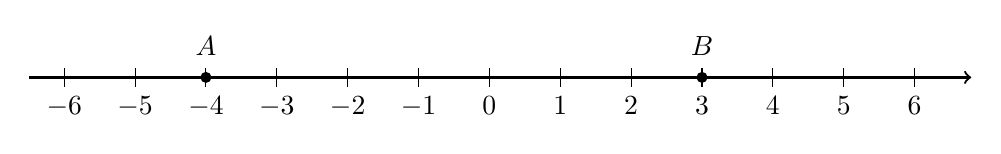
\begin{tikzpicture}[x=0.9cm,y=1cm]
    \draw[->,thick] (-6.5,0) -- (6.8,0);

    \foreach \x in {-6,-5,...,6}{
        \draw (\x,0.12) -- (\x,-0.12);
        \node[below] at (\x,-0.12) {\(\x\)};
    }

    \fill (-4,0) circle (2pt);
    \fill (3,0) circle (2pt);

    \node[above] at (-4,0.15) {\(A\)};
    \node[above] at (3,0.15) {\(B\)};
\end{tikzpicture}
\end{center}

Op een getallenas worden de getallen groter wanneer je naar
\textbf{rechts} gaat en kleiner wanneer je naar \textbf{links} gaat.

In de figuur ligt \(3\) dus rechts van \(-4\). Daarom geldt

\[
-4<3.
\]

De getallenas maakt ook duidelijk dat \(0\) de grens vormt tussen
negatieve en positieve getallen.


% ============================================================
% TEGENGESTELDE GETALLEN
% ============================================================

\FVDsubsection{Tegengestelde getallen}

Twee getallen die even ver van \(0\) liggen, maar aan verschillende kanten
van \(0\), noemen we \textbf{tegengestelde getallen}.

Zo zijn \(4\) en \(-4\) tegengesteld.

\begin{center}
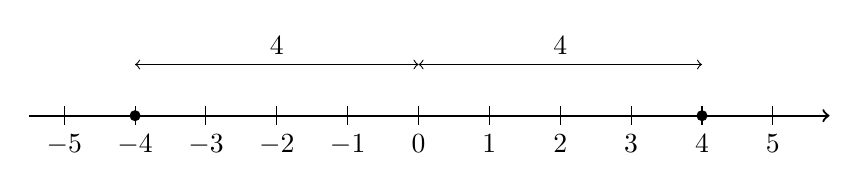
\begin{tikzpicture}[x=0.9cm,y=1cm]
    \draw[->,thick] (-5.5,0) -- (5.8,0);

    \foreach \x in {-5,-4,...,5}{
        \draw (\x,0.12) -- (\x,-0.12);
        \node[below] at (\x,-0.12) {\(\x\)};
    }

    \fill (-4,0) circle (2pt);
    \fill (4,0) circle (2pt);

    \draw[<->] (-4,0.65) -- (0,0.65);
    \draw[<->] (0,0.65) -- (4,0.65);

    \node[above] at (-2,0.65) {\(4\)};
    \node[above] at (2,0.65) {\(4\)};
\end{tikzpicture}
\end{center}

Het tegengestelde van \(7\) is \(-7\).

Het tegengestelde van \(-12\) is \(12\).

\begin{oefening}{\oefB}

Geef telkens het tegengestelde getal.

\begin{question} Het tegengestelde van \(8\) is \(\answer{-8}\). \end{question}

\begin{question} Het tegengestelde van \(-15\) is \(\answer{15}\). \end{question}

\begin{question} Het tegengestelde van \(27\) is \(\answer{-27}\). \end{question}

\begin{question} Het tegengestelde van \(-103\) is \(\answer{103}\). \end{question}

\end{oefening}


% ============================================================
% ABSOLUTE WAARDE
% ============================================================

\FVDsubsection{Absolute waarde}

Soms interesseert niet de richting, maar alleen de \textbf{afstand}.

De afstand van een getal tot \(0\) noemen we zijn
\textbf{absolute waarde}.

We schrijven bijvoorbeeld

\[
|5|=5
\]

en

\[
|-5|=5.
\]

Beide getallen liggen immers \(5\) eenheden van \(0\).

\begin{oefening}{\oefB}

Bepaal de absolute waarde.

\begin{question} \(|9|=\answer{9}\) \end{question}

\begin{question} \(|-9|=\answer{9}\) \end{question}

\begin{question} \(|-23|=\answer{23}\) \end{question}

\begin{question} \(|0|=\answer{0}\) \end{question}

\end{oefening}


% ============================================================
% TOEPASSINGEN
% ============================================================

\FVDsubsection{Getallen in toepassingen}

Positieve en negatieve getallen krijgen hun betekenis altijd vanuit een
gekozen referentiepunt. In digitale toepassingen is dat vaak een oorsprong
of een beginpositie.


\begin{oefening}[Positie in een gamewereld]{\oefB\ESS}

Een personage bevindt zich op de horizontale positie \(x=-6\).
Het beweegt \(10\) eenheden naar rechts.

\begin{question}
De nieuwe positie is \(x=\answer{4}\).
\end{question}

\end{oefening}


\begin{oefening}[Een camera verplaatsen]{\oefB}

Een camera staat op positie \(x=12\).
Ze wordt \(17\) eenheden naar links verplaatst.

\begin{question}
De nieuwe \(x\)-coördinaat is \(\answer{-5}\).
\end{question}

\end{oefening}


\begin{oefening}[Afstand tot de oorsprong]{\oefB}

Twee objecten hebben als \(x\)-coördinaat

\[
x_A=-18
\qquad\text{en}\qquad
x_B=7.
\]

\begin{question}
Object \(A\) ligt \(\answer{18}\) eenheden van de oorsprong.
\end{question}

\begin{question}
Object \(B\) ligt \(\answer{7}\) eenheden van de oorsprong.
\end{question}

\end{oefening}


\begin{oefening}[Van positie naar verplaatsing]{\oefU}

Een object bevindt zich eerst op \(x=-8\) en later op \(x=13\).

\begin{question}

Hoeveel eenheden en in welke richting is het object verplaatst?

\begin{oplossing}

De verandering van de positie is

\[
13-(-8)=21.
\]

Het object is dus \(21\) eenheden naar rechts verplaatst.

\end{oplossing}

\end{question}

\end{oefening}

    % ============================================================
% EXTRA OEFENINGEN -- GETALLEN EN GETALLENAS
% ============================================================

\begin{oefening}[Aflezen op de getallenas]{\oefB\ESS}

    Gebruik de getallenas uit de theorie.
    
    \begin{question}
    Welk getal ligt \(4\) plaatsen rechts van \(0\)?
    \(\answer{4}\)
    \end{question}
    
    \begin{question}
    Welk getal ligt \(6\) plaatsen links van \(0\)?
    \(\answer{-6}\)
    \end{question}
    
    \begin{question}
    Je start bij \(-3\) en gaat \(5\) plaatsen naar rechts.
    Je komt uit bij \(\answer{2}\).
    \end{question}
    
    \begin{question}
    Je start bij \(4\) en gaat \(7\) plaatsen naar links.
    Je komt uit bij \(\answer{-3}\).
    \end{question}
    
    \begin{question}
    Je start bij \(-5\) en gaat \(3\) plaatsen naar links.
    Je komt uit bij \(\answer{-8}\).
    \end{question}
    
    \begin{question}
    Je start bij \(-7\) en eindigt bij \(2\).
    Je bent \(\answer{9}\) plaatsen naar rechts gegaan.
    \end{question}
    
    \end{oefening}
    
    
    \begin{oefening}[Links of rechts?]{\oefB}
    
    Vul \(<\) of \(>\) in. Denk aan de positie van de getallen op de getallenas.

    \begin{multicols}{2}
        
  
    
    \begin{question} \(-3\ \answer{<}\ 2\) \end{question}
    
    \begin{question} \(5\ \answer{>}\ -4\) \end{question}
    
    \begin{question} \(-8\ \answer{<}\ -2\) \end{question}
    
    \begin{question} \(-1\ \answer{>}\ -6\) \end{question}
    
    \begin{question} \(0\ \answer{>}\ -9\) \end{question}
    
    \begin{question} \(-12\ \answer{<}\ 0\) \end{question}
\end{multicols}
    
    \end{oefening}
    
    
    \begin{oefening}[Tegengestelde getallen]{\oefB\ESS}
    
    Geef telkens het tegengestelde getal.

    \begin{multicols}{2}
          
    \begin{question} Het tegengestelde van \(12\) is \(\answer{-12}\). \end{question}
    
    \begin{question} Het tegengestelde van \(-7\) is \(\answer{7}\). \end{question}
    
    \begin{question} Het tegengestelde van \(35\) is \(\answer{-35}\). \end{question}
    
    \begin{question} Het tegengestelde van \(-48\) is \(\answer{48}\). \end{question}
    
    \begin{question} Het tegengestelde van \(100\) is \(\answer{-100}\). \end{question}
    
    \begin{question} Het tegengestelde van \(-250\) is \(\answer{250}\). \end{question}
    
    \begin{question} Het tegengestelde van \(0\) is \(\answer{0}\). \end{question}
    
    \end{multicols}

    \end{oefening}
    

    \begin{oefening}[Absolute waarde]{\oefB\ESS}
    
    Bepaal de absolute waarde.
    
    \begin{multicols}{2}
        
    \begin{question} \(|6|=\answer{6}\) \end{question}
    
    \begin{question} \(|-6|=\answer{6}\) \end{question}
    
    \begin{question} \(|17|=\answer{17}\) \end{question}
    
    \begin{question} \(|-24|=\answer{24}\) \end{question}
    
    \begin{question} \(|-105|=\answer{105}\) \end{question}
    
    \begin{question} \(|0|=\answer{0}\) \end{question}

    \end{multicols}
    
    \end{oefening}
    
    
    \begin{oefening}[Waar ligt het getal?]{\oefB}
    
    \begin{question}
    Een getal ligt \(8\) eenheden links van \(0\).
    Het getal is \(\answer{-8}\).
    \end{question}
    
    \begin{question}
    Een getal ligt \(13\) eenheden rechts van \(0\).
    Het getal is \(\answer{13}\).
    \end{question}
    
    \begin{question}
    Een getal heeft absolute waarde \(9\) en ligt links van \(0\).
    Het getal is \(\answer{-9}\).
    \end{question}
    
    \begin{question}
    Een getal heeft absolute waarde \(21\) en is positief.
    Het getal is \(\answer{21}\).
    \end{question}
    
    \end{oefening}
    
    
    % ============================================================
    % TOEPASSINGEN
    % ============================================================
    
    \begin{oefening}[Een personage bewegen]{\oefB\ESS}
    
    Een personage staat op positie \(x=-12\).
    
    \begin{question}
    Het personage beweegt \(7\) eenheden naar rechts.
    De nieuwe positie is \(x=\answer{-5}\).
    \end{question}
    
    \begin{question}
    Vanuit die nieuwe positie beweegt het nog \(9\) eenheden naar rechts.
    De nieuwe positie is \(x=\answer{4}\).
    \end{question}
    
    \begin{question}
    Hoeveel eenheden ligt de eindpositie van de oorsprong?
    \(\answer{4}\)
    \end{question}
    
    \end{oefening}
    
    
    \begin{oefening}[Camera in een 3D-scène]{\oefB}
    
    In een 3D-scène gebruiken we een \(x\)-as.
    Een camera bevindt zich op \(x=-15\).
    
    \begin{question}
    De camera wordt \(20\) eenheden naar rechts verplaatst.
    De nieuwe positie is \(x=\answer{5}\).
    \end{question}
    
    \begin{question}
    Hoe ver ligt de camera nu van \(x=0\)?
    \(\answer{5}\) eenheden.
    \end{question}
    
    \end{oefening}
    
    
    \begin{oefening}[Verdiepingen]{\oefB}
    
    In een gebouw noemen we het gelijkvloers niveau \(0\).
    Ondergrondse verdiepingen krijgen een negatief nummer.
    
    Een lift staat op niveau \(-3\).
    
    \begin{question}
    De lift stijgt \(5\) verdiepingen.
    Ze komt aan op niveau \(\answer{2}\).
    \end{question}
    
    \begin{question}
    Hoeveel verdiepingen heeft de lift afgelegd?
    \(\answer{5}\)
    \end{question}
    
    \end{oefening}
    
    
    \begin{oefening}[Temperatuurverschil]{\oefB}
    
    's Nachts is de temperatuur \(-6^\circ\text{C}\).
    Overdag stijgt de temperatuur tot \(4^\circ\text{C}\).
    
    \begin{question}
    Met hoeveel graden is de temperatuur gestegen?
    \(\answer{10}^\circ\text{C}\)
    \end{question}
    
    \end{oefening}
    
    
    \begin{oefening}[Objecten rond de oorsprong]{\oefU}
    
    Drie objecten bevinden zich op een horizontale as:
    
    \[
    x_A=-12,
    \qquad
    x_B=5,
    \qquad
    x_C=-3.
    \]
    
    \begin{question}
    Welk object ligt het dichtst bij de oorsprong?
    
    \begin{multipleChoice}
        \choice{Object \(A\)}
        \choice{Object \(B\)}
        \choice[correct]{Object \(C\)}
    \end{multipleChoice}
    \end{question}
    
    \begin{question}
    Hoe ver ligt object \(A\) van de oorsprong?
    \(\answer{12}\) eenheden.
    \end{question}
    
    \begin{question}
    Hoe ver liggen \(A\) en \(B\) van elkaar?
    \(\answer{17}\) eenheden.
    \end{question}
    
    \end{oefening}
    
    
    \begin{oefening}[Van positie naar verplaatsing]{\oefU\ESS}
    
    Een gameobject begint op \(x=-14\) en eindigt op \(x=9\).
    
    \begin{question}
    
    Bepaal de verplaatsing en leg uit hoe je die vindt.
    
    \begin{oplossing}
    
    We berekenen de eindpositie min de beginpositie:
    
    \[
    9-(-14)=23.
    \]
    
    De verplaatsing is dus \(23\) eenheden naar rechts.
    
    \end{oplossing}
    
    \end{question}
    
    \end{oefening}
    
    
    \begin{oefening}[Zelf een positie reconstrueren]{\oefU}
    
    Een object wordt \(18\) eenheden naar rechts verplaatst en eindigt op
    \(x=7\).
    
    \begin{question}
    
    Op welke positie stond het object oorspronkelijk?
    
    \begin{oplossing}
    
    We zoeken een getal waarvoor
    
    \[
    x+18=7.
    \]
    
    Dus
    
    \[
    x=7-18=-11.
    \]
    
    Het object stond oorspronkelijk op \(x=-11\).
    
    \end{oplossing}
    
    \end{question}
    
    \end{oefening}

    % ============================================================
% GEVORDERDE OEFENINGEN
% ============================================================

\begin{oefening}[Twee bewegende objecten]{\oefG}

    Twee objecten bewegen langs dezelfde horizontale as.
    
    Object \(A\) start op \(x=-18\) en beweegt \(27\) eenheden naar rechts.
    Object \(B\) start op \(x=16\) en beweegt \(11\) eenheden naar links.
    
    \begin{question}
    
    Bepaal de eindpositie van beide objecten en bereken hoe ver ze daarna
    van elkaar verwijderd zijn.
    
    \begin{oplossing}
    
    Voor object \(A\):
    
    \[
    -18+27=9.
    \]
    
    Dus
    
    \[
    x_A=9.
    \]
    
    Voor object \(B\):
    
    \[
    16-11=5.
    \]
    
    Dus
    
    \[
    x_B=5.
    \]
    
    De afstand tussen beide objecten is
    
    \[
    |9-5|=4.
    \]
    
    De objecten bevinden zich uiteindelijk dus \(4\) eenheden van elkaar.
    
    \end{oplossing}
    
    \end{question}
    
    \end{oefening}
    
    
    \begin{oefening}[Waar stond de camera?]{\oefG\ESS}
    
    Een camera beweegt langs de \(x\)-as.
    
    Eerst wordt ze \(14\) eenheden naar links verplaatst.
    Daarna wordt ze \(9\) eenheden naar rechts verplaatst.
    De camera eindigt op \(x=-8\).
    
    \begin{question}
    
    Bepaal de oorspronkelijke positie van de camera.
    
    \begin{oplossing}
    
    De totale verandering is
    
    \[
    -14+9=-5.
    \]
    
    De camera eindigt dus \(5\) eenheden links van haar oorspronkelijke
    positie.
    
    Als \(x\) de oorspronkelijke positie is, dan geldt
    
    \[
    x-5=-8.
    \]
    
    Daaruit volgt
    
    \[
    x=-3.
    \]
    
    De camera stond oorspronkelijk op
    
    \[
    x=-3.
    \]
    
    Controle:
    
    \[
    -3-14=-17
    \]
    
    en vervolgens
    
    \[
    -17+9=-8.
    \]
    
    Dit is inderdaad de gegeven eindpositie.
    
    \end{oplossing}
    
    \end{question}
    
    \end{oefening}
    
    
    \begin{oefening}[Een symmetrische gamewereld]{\oefG}
    
    In een gamewereld ligt een controlepunt op \(x=0\).
    
    Twee objecten \(A\) en \(B\) liggen aan verschillende kanten van dit
    controlepunt. Ze liggen precies \(34\) eenheden van elkaar.
    
    Object \(A\) bevindt zich op \(x=-11\).
    
    \begin{question}
    
    Bepaal de positie van object \(B\).
    
    \begin{oplossing}
    
    Object \(A\) ligt \(11\) eenheden links van het controlepunt.
    
    Omdat \(A\) en \(B\) aan verschillende kanten van \(0\) liggen, bestaat
    de totale afstand uit twee delen:
    
    \[
    11+\text{afstand van }B\text{ tot }0=34.
    \]
    
    Daarom is de afstand van \(B\) tot \(0\)
    
    \[
    34-11=23.
    \]
    
    Object \(B\) ligt aan de positieve kant van de getallenas, dus
    
    \[
    x_B=23.
    \]
    
    Controle:
    
    \[
    |23-(-11)|=|34|=34.
    \]
    
    \end{oplossing}
    
    \end{question}
    
    \end{oefening}
    
    \begin{oefening}[De metrotunnel]{\oefG\ESS}

        Voor een game wordt een verlaten metrotunnel ontworpen.
        We bekijken de tunnel voorlopig als één lange horizontale lijn.
        
        Het midden van het oude station wordt gekozen als oorsprong:
        
        \[
        x=0.
        \]
        
        Posities rechts van het station zijn positief en posities links van het
        station zijn negatief.
        
        Bij de start van het level bevindt de speler zich op
        
        \[
        x=-35.
        \]
        
        In de tunnel staan drie belangrijke objecten:
        
        \[
        \text{controlepost } C: x=-12,
        \qquad
        \text{generator } G: x=18,
        \qquad
        \text{uitgang } U: x=47.
        \]
        
        De speler moet eerst de controlepost bereiken, daarna de generator
        activeren en ten slotte naar de uitgang gaan.
        
        
        \begin{question}
        
        Teken een getallenas en duid daarop de oorsprong, de startpositie van de
        speler en de drie belangrijke objecten aan.
        
        \begin{oplossing}
        
        Op de getallenas liggen de punten van links naar rechts op
        
        \[
        -35,\qquad -12,\qquad 0,\qquad 18,\qquad 47.
        \]
        
        De startpositie ligt dus links van de controlepost. De generator en de
        uitgang liggen rechts van de oorsprong.
        
        \end{oplossing}
        
        \end{question}
        
        
        \begin{question}
        
        Hoeveel eenheden moet de speler afleggen om van zijn startpositie naar de
        controlepost te gaan? Geef ook de richting.
        
        \begin{oplossing}
        
        De speler gaat van \(-35\) naar \(-12\).
        
        De verplaatsing is
        
        \[
        -12-(-35)=23.
        \]
        
        De speler beweegt dus \(23\) eenheden naar rechts.
        
        \end{oplossing}
        
        \end{question}
        
        
        \begin{question}
        
        Na de controlepost gaat de speler verder naar de generator.
        Hoeveel eenheden legt hij tijdens dit tweede deel af?
        
        \begin{oplossing}
        
        De speler gaat van \(-12\) naar \(18\).
        
        \[
        18-(-12)=30.
        \]
        
        Hij legt dus \(30\) eenheden af.
        
        \end{oplossing}
        
        \end{question}
        
        
        \begin{question}
        
        Na het activeren van de generator loopt de speler naar de uitgang.
        Bereken de afstand van de generator tot de uitgang.
        
        \begin{oplossing}
        
        \[
        47-18=29.
        \]
        
        De afstand bedraagt dus \(29\) eenheden.
        
        \end{oplossing}
        
        \end{question}
        
        
        \begin{question}
        
        Hoeveel eenheden heeft de speler in totaal afgelegd vanaf zijn
        startpositie tot aan de uitgang?
        
        \begin{oplossing}
        
        De drie afgelegde afstanden zijn
        
        \[
        23,\qquad 30,\qquad 29.
        \]
        
        Dus
        
        \[
        23+30+29=82.
        \]
        
        De speler heeft in totaal \(82\) eenheden afgelegd.
        
        We kunnen dit ook rechtstreeks controleren. De speler beweegt voortdurend
        naar rechts, van \(-35\) tot \(47\):
        
        \[
        47-(-35)=82.
        \]
        
        Beide methodes geven hetzelfde resultaat.
        
        \end{oplossing}
        
        \end{question}
        
        
        \begin{question}
        
        De leveldesigner voegt nu een geheime kamer toe.
        
        De kamer ligt links van de oorsprong en bevindt zich \(26\) eenheden van
        het midden van het station.
        
        Bepaal de \(x\)-coördinaat van de geheime kamer.
        
        \begin{oplossing}
        
        De afstand tot de oorsprong is \(26\), dus de absolute waarde van de
        coördinaat is
        
        \[
        |x|=26.
        \]
        
        Omdat de kamer links van de oorsprong ligt, is de coördinaat negatief.
        
        Daarom:
        
        \[
        x=-26.
        \]
        
        \end{oplossing}
        
        \end{question}
        
        
        \begin{question}
        
        De speler bevindt zich bij de generator op \(x=18\) en ontdekt de geheime
        kamer op \(x=-26\).
        
        Hoe ver is het van de generator naar de geheime kamer?
        
        \begin{oplossing}
        
        De afstand tussen beide posities is
        
        \[
        |18-(-26)|
        =
        |44|
        =
        44.
        \]
        
        De geheime kamer ligt dus \(44\) eenheden van de generator.
        
        \end{oplossing}
        
        \end{question}
        
        
        \begin{question}
        
        De ontwerper wil een tweede geheime kamer plaatsen die even ver van de
        oorsprong ligt als de eerste, maar aan de andere kant van het station.
        
        Bepaal de positie van deze tweede kamer.
        
        \begin{oplossing}
        
        De eerste geheime kamer bevindt zich op
        
        \[
        x=-26.
        \]
        
        Het tegengestelde getal is
        
        \[
        26.
        \]
        
        De tweede kamer moet dus op
        
        \[
        x=26
        \]
        
        worden geplaatst.
        
        Beide kamers liggen \(26\) eenheden van de oorsprong:
        
        \[
        |-26|=|26|=26.
        \]
        
        \end{oplossing}
        
        \end{question}
        
        
        \begin{question}
        
        Een tester beweert:
        
        \begin{quote}
        ``De speler legt van de startpositie \(x=-35\) tot de uitgang \(x=47\)
        maar \(47-35=12\) eenheden af.''
        \end{quote}
        
        Leg uit wat er fout is aan deze redenering en geef de correcte berekening.
        
        \begin{oplossing}
        
        De startpositie is niet \(35\), maar \(-35\).
        
        We moeten dus het verschil berekenen tussen \(47\) en \(-35\):
        
        \[
        47-(-35)=47+35=82.
        \]
        
        Op een getallenas zien we hetzelfde: van \(-35\) tot \(0\) zijn er
        \(35\) eenheden en van \(0\) tot \(47\) nog eens \(47\) eenheden.
        
        Dus
        
        \[
        35+47=82.
        \]
        
        De correcte afstand is \(82\) eenheden.
        
        \end{oplossing}
        
        \end{question}
        
        \end{oefening}


% ============================================================
% 5. HOOFDREKENEN ALS HERSCHRIJVEN
% ============================================================

\FVDsection{Hoofdrekenen is slim herschrijven}

Bij hoofdrekenen probeer je een moeilijke berekening om te vormen tot een
gemakkelijkere berekening.

Neem bijvoorbeeld \(
49+28.
\)

Je kan rechtstreeks rekenen, maar ook:
\(
49+28
=
50+28-1
=
77.
\)

Bij

\(
25\cdot16
\)

kan je denken:
\(
25\cdot16
=
100\cdot4
=
400.
\)
Een goede hoofdrekenstrategie maakt gebruik van de structuur van de getallen.

Belangrijke strategieën zijn:
\begin{multicols}{2}
    \begin{itemize}
    \item splitsen;
    \item aanvullen;
    \item compenseren;
    \item handig groeperen;
    \item verdubbelen en halveren;
    \item een omgekeerde bewerking gebruiken.
\end{itemize}
\end{multicols}

% ============================================================
% 6. HANDIG OPTELLEN
% ============================================================

\FVDsubsection{Handig optellen}


% ------------------------------------------------------------
% SPLITSEN
% ------------------------------------------------------------

\subsubsection*{Splitsen}

Je kan een getal opsplitsen in tientallen, honderdtallen of andere handige
delen.

\begin{voorbeeld}

Bereken:

\[
47+36.
\]

Splits \(36\) in \(30+6\):

\[
47+36
=
47+30+6
=
77+6
=
83.
\]

\end{voorbeeld}


\begin{voorbeeld}

Bereken:

\[
325+148.
\]

\[
325+148
=
325+100+40+8
=
425+40+8
=
473.
\]

\end{voorbeeld}


\begin{oefening}[Optellen door te splitsen]{\oefB\ESS}

    Bereken zonder rekenmachine. Splits een van de getallen in handige delen.
    
    \begin{multicols}{3}
    
    \begin{question} \(34+25=\answer{59}\) \end{question}
    
    \begin{question} \(47+32=\answer{79}\) \end{question}
    
    \begin{question} \(52+36=\answer{88}\) \end{question}
    
    \begin{question} \(63+24=\answer{87}\) \end{question}
    
    \begin{question} \(58+26=\answer{84}\) \end{question}
    
    \begin{question} \(71+38=\answer{109}\) \end{question}
    
    \begin{question} \(46+57=\answer{103}\) \end{question}
    
    \begin{question} \(73+48=\answer{121}\) \end{question}
    
    \begin{question} \(85+67=\answer{152}\) \end{question}
    
    \begin{question} \(96+78=\answer{174}\) \end{question}
    
    \begin{question} \(125+46=\answer{171}\) \end{question}
    
    \begin{question} \(214+73=\answer{287}\) \end{question}
    
    \begin{question} \(326+58=\answer{384}\) \end{question}
    
    \begin{question} \(238+157=\answer{395}\) \end{question}
    
    \begin{question} \(354+128=\answer{482}\) \end{question}
    
    \begin{question} \(427+265=\answer{692}\) \end{question}
    
    \begin{question} \(475+328=\answer{803}\) \end{question}
    
    \begin{question} \(586+247=\answer{833}\) \end{question}
    
    \begin{question} \(638+175=\answer{813}\) \end{question}
    
    \begin{question} \(746+189=\answer{935}\) \end{question}
    
    \begin{question} \(1230+450=\answer{1680}\) \end{question}
    
    \begin{question} \(1525+340=\answer{1865}\) \end{question}
    
    \begin{question} \(1835+720=\answer{2555}\) \end{question}
    
    \begin{question} \(2410+680=\answer{3090}\) \end{question}
    
    \begin{question} \(3504+287=\answer{3791}\) \end{question}
    
    \begin{question} \(4260+375=\answer{4635}\) \end{question}
    
    \begin{question} \(5125+748=\answer{5873}\) \end{question}
    
    \begin{question} \(4620+1380=\answer{6000}\) \end{question}
    
    \begin{question} \(6750+1245=\answer{7995}\) \end{question}
    
    \begin{question} \(8235+1768=\answer{10003}\) \end{question}
    
    \end{multicols}
    
    \end{oefening}


% ------------------------------------------------------------
% AANVULLEN
% ------------------------------------------------------------

\subsubsection*{Aanvullen tot een rond getal}

Bij

\[
68+27
\]

kan je eerst \(68\) aanvullen tot \(70\).

Daarvoor gebruik je \(2\) van de \(27\):

\[
68+27
=
68+2+25
=
70+25
=
95.
\]


\begin{oefening}[Maak eerst een rond getal]{\oefB\ESS}

    Bereken handig. Vul eerst aan tot een rond getal.
    
    \begin{multicols}{3}
    
    \begin{question} \(39+26=\answer{65}\) \end{question}
    
    \begin{question} \(48+35=\answer{83}\) \end{question}
    
    \begin{question} \(57+24=\answer{81}\) \end{question}
    
    \begin{question} \(67+28=\answer{95}\) \end{question}
    
    \begin{question} \(78+46=\answer{124}\) \end{question}
    
    \begin{question} \(89+37=\answer{126}\) \end{question}
    
    \begin{question} \(58+27=\answer{85}\) \end{question}
    
    \begin{question} \(76+38=\answer{114}\) \end{question}
    
    \begin{question} \(87+55=\answer{142}\) \end{question}
    
    \begin{question} \(96+47=\answer{143}\) \end{question}
    
    \begin{question} \(195+37=\answer{232}\) \end{question}
    
    \begin{question} \(294+58=\answer{352}\) \end{question}
    
    \begin{question} \(387+46=\answer{433}\) \end{question}
    
    \begin{question} \(496+27=\answer{523}\) \end{question}
    
    \begin{question} \(598+35=\answer{633}\) \end{question}
    
    \begin{question} \(697+48=\answer{745}\) \end{question}
    
    \begin{question} \(795+67=\answer{862}\) \end{question}
    
    \begin{question} \(894+39=\answer{933}\) \end{question}
    
    \begin{question} \(997+56=\answer{1053}\) \end{question}
    
    \begin{question} \(1195+78=\answer{1273}\) \end{question}
    
    \begin{question} \(1497+65=\answer{1562}\) \end{question}
    
    \begin{question} \(1998+37=\answer{2035}\) \end{question}
    
    \begin{question} \(2396+128=\answer{2524}\) \end{question}
    
    \begin{question} \(2997+84=\answer{3081}\) \end{question}
    
    \begin{question} \(3495+217=\answer{3712}\) \end{question}
    
    \begin{question} \(3998+156=\answer{4154}\) \end{question}
    
    \begin{question} \(4997+214=\answer{5211}\) \end{question}
    
    \begin{question} \(5996+328=\answer{6324}\) \end{question}
    
    \begin{question} \(7998+475=\answer{8473}\) \end{question}
    
    \begin{question} \(9997+628=\answer{10625}\) \end{question}
    
    \end{multicols}
    
    \end{oefening}


% ------------------------------------------------------------
% COMPENSEREN
% ------------------------------------------------------------

\subsubsection*{Compenseren}

Sommige getallen liggen heel dicht bij een rond getal.

Bijvoorbeeld:

\[
199=200-1.
\]

Daarom:

\[
347+199
=
347+200-1
=
546.
\]


\begin{voorbeeld}

\[
598+275
=
600+275-2
=
873.
\]

\end{voorbeeld}


\begin{oefening}[Compenseren bij optellen]{\oefB\ESS}

    Bereken handig door een getal tijdelijk te vervangen door een nabijgelegen
    rond getal en daarna te compenseren.
    
    \begin{multicols}{3}
    
    \begin{question} \(36+19=\answer{55}\) \end{question}
    
    \begin{question} \(47+29=\answer{76}\) \end{question}
    
    \begin{question} \(58+39=\answer{97}\) \end{question}
    
    \begin{question} \(64+49=\answer{113}\) \end{question}
    
    \begin{question} \(75+59=\answer{134}\) \end{question}
    
    \begin{question} \(83+98=\answer{181}\) \end{question}
    
    \begin{question} \(126+99=\answer{225}\) \end{question}
    
    \begin{question} \(245+99=\answer{344}\) \end{question}
    
    \begin{question} \(317+199=\answer{516}\) \end{question}
    
    \begin{question} \(378+199=\answer{577}\) \end{question}
    
    \begin{question} \(526+298=\answer{824}\) \end{question}
    
    \begin{question} \(684+299=\answer{983}\) \end{question}
    
    \begin{question} \(875+399=\answer{1274}\) \end{question}
    
    \begin{question} \(437+498=\answer{935}\) \end{question}
    
    \begin{question} \(596+499=\answer{1095}\) \end{question}
    
    \begin{question} \(725+598=\answer{1323}\) \end{question}
    
    \begin{question} \(799+426=\answer{1225}\) \end{question}
    
    \begin{question} \(846+999=\answer{1845}\) \end{question}
    
    \begin{question} \(1240+998=\answer{2238}\) \end{question}
    
    \begin{question} \(1575+999=\answer{2574}\) \end{question}
    
    \begin{question} \(1999+876=\answer{2875}\) \end{question}
    
    \begin{question} \(2385+1998=\answer{4383}\) \end{question}
    
    \begin{question} \(3997+208=\answer{4205}\) \end{question}
    
    \begin{question} \(4250+2999=\answer{7249}\) \end{question}
    
    \begin{question} \(5784+3998=\answer{9782}\) \end{question}
    
    \begin{question} \(6245+4999=\answer{11244}\) \end{question}
    
    \begin{question} \(7998+1357=\answer{9355}\) \end{question}
    
    \begin{question} \(8640+5999=\answer{14639}\) \end{question}
    
    \begin{question} \(9998+604=\answer{10602}\) \end{question}
    
    \begin{question} \(12750+9999=\answer{22749}\) \end{question}
    
    \end{multicols}
    
    \end{oefening}


% ------------------------------------------------------------
% GROEPEREN
% ------------------------------------------------------------

\subsubsection*{Handig groeperen}

Wanneer verschillende getallen worden opgeteld, kan de volgorde waarin je
rekent veel verschil maken.

\begin{voorbeeld}

Bereken:

\[
18+37+82+63.
\]

We groeperen:

\[
18+82=100
\]

en

\[
37+63=100.
\]

Dus

\[
18+37+82+63=200.
\]

\end{voorbeeld}


\begin{oefening}[Handig groeperen]{\oefB\ESS}

    Bereken zo efficiënt mogelijk. Zoek eerst getallen die samen een handig
    rond getal vormen.
    
    \begin{multicols}{2}
    
    \begin{question} \(20+35+80+65=\answer{200}\) \end{question}
    
    \begin{question} \(25+48+75+52=\answer{200}\) \end{question}
    
    \begin{question} \(17+29+71+83=\answer{200}\) \end{question}
    
    \begin{question} \(32+68+41+59=\answer{200}\) \end{question}
    
    \begin{question} \(13+87+26+74=\answer{200}\) \end{question}
    
    \begin{question} \(44+56+38+62=\answer{200}\) \end{question}
    
    \begin{question} \(125+75+240+260=\answer{700}\) \end{question}
    
    \begin{question} \(150+350+225+275=\answer{1000}\) \end{question}
    
    \begin{question} \(125+375+240+260=\answer{1000}\) \end{question}
    
    \begin{question} \(450+175+50+325=\answer{1000}\) \end{question}
    
    \begin{question} \(315+185+420+80=\answer{1000}\) \end{question}
    
    \begin{question} \(275+225+340+160=\answer{1000}\) \end{question}
    
    \begin{question} \(490+510+175+825=\answer{2000}\) \end{question}
    
    \begin{question} \(250+340+750+660=\answer{2000}\) \end{question}
    
    \begin{question} \(625+375+480+520=\answer{2000}\) \end{question}
    
    \begin{question} \(735+265+410+590=\answer{2000}\) \end{question}
    
    \begin{question} \(120+380+225+275=\answer{1000}\) \end{question}
    
    \begin{question} \(145+355+190+310=\answer{1000}\) \end{question}
    
    \begin{question} \(18+82+27+73+35+65=\answer{300}\) \end{question}
    
    \begin{question} \(14+86+39+61+42+58=\answer{300}\) \end{question}
    
    \begin{question} \(125+875+240+760+350+650=\answer{3000}\) \end{question}
    
    \begin{question} \(175+825+430+570+290+710=\answer{3000}\) \end{question}
    
    \begin{question} \(225+775+315+685+440+560=\answer{3000}\) \end{question}
    
    \begin{question} \(480+520+725+275+630+370=\answer{3000}\) \end{question}
    
    \begin{question} \(1250+750+640+360=\answer{3000}\) \end{question}
    
    \begin{question} \(1450+550+875+125=\answer{3000}\) \end{question}
    
    \begin{question} \(2350+650+1425+575=\answer{5000}\) \end{question}
    
    \begin{question} \(1750+1250+860+1140=\answer{5000}\) \end{question}
    
    \begin{question} \(2750+250+1625+375=\answer{5000}\) \end{question}
    
    \begin{question} \(3480+520+1275+725=\answer{6000}\) \end{question}
    
    \end{multicols}
    
    \end{oefening}


% ------------------------------------------------------------
% GEMENGD
% ------------------------------------------------------------

\begin{oefening}[Kies zelf een optelstrategie]{\oefU\ESS}

    Bereken zonder rekenmachine.
    
    Je krijgt niet meer te horen welke strategie je moet gebruiken.
    Probeer telkens een efficiënte strategie te kiezen.
    
    \begin{multicols}{2}
    
    \begin{question} \(69+47=\answer{116}\) \end{question}
    
    \begin{question} \(58+36=\answer{94}\) \end{question}
    
    \begin{question} \(87+48=\answer{135}\) \end{question}
    
    \begin{question} \(125+68=\answer{193}\) \end{question}
    
    \begin{question} \(298+47=\answer{345}\) \end{question}
    
    \begin{question} \(398+125=\answer{523}\) \end{question}
    
    \begin{question} \(245+199=\answer{444}\) \end{question}
    
    \begin{question} \(497+86=\answer{583}\) \end{question}
    
    \begin{question} \(699+248=\answer{947}\) \end{question}
    
    \begin{question} \(499+399=\answer{898}\) \end{question}
    
    \begin{question} \(125+375+48+52=\answer{600}\) \end{question}
    
    \begin{question} \(37+63+28+72=\answer{200}\) \end{question}
    
    \begin{question} \(275+199+25=\answer{499}\) \end{question}
    
    \begin{question} \(348+652+125=\answer{1125}\) \end{question}
    
    \begin{question} \(175+325+240+260=\answer{1000}\) \end{question}
    
    \begin{question} \(596+278=\answer{874}\) \end{question}
    
    \begin{question} \(798+357=\answer{1155}\) \end{question}
    
    \begin{question} \(997+648=\answer{1645}\) \end{question}
    
    \begin{question} \(1498+375=\answer{1873}\) \end{question}
    
    \begin{question} \(1998+768=\answer{2766}\) \end{question}
    
    \begin{question} \(475+525+368=\answer{1368}\) \end{question}
    
    \begin{question} \(625+375+148+252=\answer{1400}\) \end{question}
    
    \begin{question} \(1499+786=\answer{2285}\) \end{question}
    
    \begin{question} \(2398+475=\answer{2873}\) \end{question}
    
    \begin{question} \(2997+856=\answer{3853}\) \end{question}
    
    \begin{question} \(1750+250+625+375=\answer{3000}\) \end{question}
    
    \begin{question} \(3998+1247=\answer{5245}\) \end{question}
    
    \begin{question} \(2499+1998=\answer{4497}\) \end{question}
    
    \begin{question} \(2750+1250+675+325=\answer{5000}\) \end{question}
    
    \begin{question} \(4997+2386=\answer{7383}\) \end{question}
    
    \end{multicols}
    
    \end{oefening}


    \begin{oefening}[Gevorderd hoofdrekenen -- optellen boven \(1000\)]{\oefG}

        Bereken zonder rekenmachine.
        
        De getallen zijn groter, maar de strategieën blijven dezelfde.
        Zoek naar ronde getallen, handige koppels en mogelijkheden om te
        compenseren. Schrijf tussenstappen op wanneer dat helpt.
        
        \begin{multicols}{2}
        
        \begin{question}
        \(2450+1750=\answer{4200}\)
        \end{question}
        
        \begin{question}
        \(3750+2480=\answer{6230}\)
        \end{question}
        
        \begin{question}
        \(4998+2750=\answer{7748}\)
        \end{question}
        
        \begin{question}
        \(6997+1850=\answer{8847}\)
        \end{question}
        
        \begin{question}
        \(9998+3475=\answer{13473}\)
        \end{question}
        
        \begin{question}
        \(12450+2998=\answer{15448}\)
        \end{question}
        
        \begin{question}
        \(4750+5250+875=\answer{10875}\)
        \end{question}
        
        \begin{question}
        \(2750+1250+3680=\answer{7680}\)
        \end{question}
        
        \begin{question}
        \(6250+3750+1480=\answer{11480}\)
        \end{question}
        
        \begin{question}
        \(4750+2250+3250+1750=\answer{12000}\)
        \end{question}
        
        \begin{question}
        \(3998+5997=\answer{9995}\)
        \end{question}
        
        \begin{question}
        \(7999+4998=\answer{12997}\)
        \end{question}
        
        \begin{question}
        \(14998+6997=\answer{21995}\)
        \end{question}
        
        \begin{question}
        \(24999+12998=\answer{37997}\)
        \end{question}
        
        \begin{question}
        \(8750+1250+4675+325=\answer{15000}\)
        \end{question}
        
        \begin{question}
        \(1275+3725+6480+3520=\answer{15000}\)
        \end{question}
        
        \begin{question}
        \(12450+7550+3875+1125=\answer{25000}\)
        \end{question}
        
        \begin{question}
        \(2498+7502+3997+6003=\answer{20000}\)
        \end{question}
        
        \begin{question}
        \(9997+4998+3003+2002=\answer{20000}\)
        \end{question}
        
        \begin{question}
        \(14999+5001+12498+7502=\answer{40000}\)
        \end{question}
        
        \end{multicols}
        
        \end{oefening}
% ============================================================
% 7. HANDIG AFTREKKEN
% ============================================================

\FVDsubsection{Handig aftrekken}


% ------------------------------------------------------------
% SPLITSEN
% ------------------------------------------------------------

\subsubsection*{Splitsen}

Bij aftrekken kan je het getal dat je aftrekt opsplitsen in handige delen.

\begin{voorbeeld}

Bereken:

\[
83-46.
\]

Splits \(46\) in \(40+6\):

\[
83-46
=
83-40-6
=
43-6
=
37.
\]

\end{voorbeeld}


\begin{oefening}[Aftrekken door te splitsen]{\oefB\ESS}

Bereken zonder rekenmachine. Splits het getal dat je aftrekt in handige delen.

\begin{multicols}{3}

\begin{question} \(75-32=\answer{43}\) \end{question}

\begin{question} \(86-43=\answer{43}\) \end{question}

\begin{question} \(92-31=\answer{61}\) \end{question}

\begin{question} \(84-52=\answer{32}\) \end{question}

\begin{question} \(97-64=\answer{33}\) \end{question}

\begin{question} \(94-57=\answer{37}\) \end{question}

\begin{question} \(83-46=\answer{37}\) \end{question}

\begin{question} \(125-68=\answer{57}\) \end{question}

\begin{question} \(143-57=\answer{86}\) \end{question}

\begin{question} \(172-86=\answer{86}\) \end{question}

\begin{question} \(235-112=\answer{123}\) \end{question}

\begin{question} \(348-126=\answer{222}\) \end{question}

\begin{question} \(426-213=\answer{213}\) \end{question}

\begin{question} \(537-324=\answer{213}\) \end{question}

\begin{question} \(684-251=\answer{433}\) \end{question}

\begin{question} \(725-413=\answer{312}\) \end{question}

\begin{question} \(803-281=\answer{522}\) \end{question}

\begin{question} \(903-481=\answer{422}\) \end{question}

\begin{question} \(964-532=\answer{432}\) \end{question}

\begin{question} \(875-647=\answer{228}\) \end{question}

\begin{question} \(1200-450=\answer{750}\) \end{question}

\begin{question} \(1450-725=\answer{725}\) \end{question}

\begin{question} \(1875-630=\answer{1245}\) \end{question}

\begin{question} \(2350-1275=\answer{1075}\) \end{question}

\begin{question} \(3280-1460=\answer{1820}\) \end{question}

\begin{question} \(5040-1820=\answer{3220}\) \end{question}

\begin{question} \(6240-2370=\answer{3870}\) \end{question}

\begin{question} \(7600-3450=\answer{4150}\) \end{question}

\begin{question} \(8425-3210=\answer{5215}\) \end{question}

\begin{question} \(9750-4635=\answer{5115}\) \end{question}

\end{multicols}

\end{oefening}


% ------------------------------------------------------------
% AANVULLEN
% ------------------------------------------------------------

\subsubsection*{Aanvullen}

Wanneer twee getallen dicht bij elkaar liggen, is het vaak gemakkelijker
om niet rechtstreeks af te trekken, maar te bepalen hoeveel je moet
\textbf{aanvullen} om van het ene getal naar het andere te gaan.

\begin{voorbeeld}

Bereken:

\[
503-487.
\]

Van \(487\) naar \(500\) is \(13\).

Van \(500\) naar \(503\) is \(3\).

Dus:

\[
503-487
=
13+3
=
16.
\]

\end{voorbeeld}


\begin{oefening}[Aftrekken door aan te vullen]{\oefB}

Bereken handig door aan te vullen.

\begin{multicols}{3}

\begin{question} \(51-47=\answer{4}\) \end{question}

\begin{question} \(63-58=\answer{5}\) \end{question}

\begin{question} \(72-66=\answer{6}\) \end{question}

\begin{question} \(84-79=\answer{5}\) \end{question}

\begin{question} \(101-96=\answer{5}\) \end{question}

\begin{question} \(104-97=\answer{7}\) \end{question}

\begin{question} \(203-189=\answer{14}\) \end{question}

\begin{question} \(302-287=\answer{15}\) \end{question}

\begin{question} \(403-388=\answer{15}\) \end{question}

\begin{question} \(503-488=\answer{15}\) \end{question}

\begin{question} \(604-589=\answer{15}\) \end{question}

\begin{question} \(705-688=\answer{17}\) \end{question}

\begin{question} \(803-789=\answer{14}\) \end{question}

\begin{question} \(904-879=\answer{25}\) \end{question}

\begin{question} \(1002-987=\answer{15}\) \end{question}

\begin{question} \(1005-978=\answer{27}\) \end{question}

\begin{question} \(1503-1487=\answer{16}\) \end{question}

\begin{question} \(2005-1998=\answer{7}\) \end{question}

\begin{question} \(2504-2489=\answer{15}\) \end{question}

\begin{question} \(3001-2984=\answer{17}\) \end{question}

\begin{question} \(4003-3978=\answer{25}\) \end{question}

\begin{question} \(5004-4979=\answer{25}\) \end{question}

\begin{question} \(6002-5987=\answer{15}\) \end{question}

\begin{question} \(7005-6978=\answer{27}\) \end{question}

\begin{question} \(8003-7989=\answer{14}\) \end{question}

\begin{question} \(9004-8976=\answer{28}\) \end{question}

\begin{question} \(10000-9987=\answer{13}\) \end{question}

\begin{question} \(12003-11986=\answer{17}\) \end{question}

\begin{question} \(15005-14978=\answer{27}\) \end{question}

\begin{question} \(20004-19979=\answer{25}\) \end{question}

\end{multicols}

\end{oefening}


% ------------------------------------------------------------
% COMPENSEREN
% ------------------------------------------------------------

\subsubsection*{Compenseren}

Ligt het getal dat je aftrekt dicht bij een rond getal, dan kan je eerst
met dat ronde getal rekenen en daarna compenseren.

\begin{voorbeeld}

Bereken:

\[
725-199.
\]

Omdat

\[
199=200-1,
\]

krijgen we:

\[
725-199
=
725-200+1
=
526.
\]

We hebben eerst \(1\) te veel afgetrokken. Daarom tellen we die \(1\)
op het einde weer bij.

\end{voorbeeld}


\begin{oefening}[Compenseren bij aftrekken]{\oefB\ESS}

Bereken handig.

\begin{multicols}{3}

\begin{question} \(150-49=\answer{101}\) \end{question}

\begin{question} \(230-99=\answer{131}\) \end{question}

\begin{question} \(450-99=\answer{351}\) \end{question}

\begin{question} \(520-198=\answer{322}\) \end{question}

\begin{question} \(725-198=\answer{527}\) \end{question}

\begin{question} \(840-199=\answer{641}\) \end{question}

\begin{question} \(640-297=\answer{343}\) \end{question}

\begin{question} \(750-299=\answer{451}\) \end{question}

\begin{question} \(1000-399=\answer{601}\) \end{question}

\begin{question} \(1205-499=\answer{706}\) \end{question}

\begin{question} \(1500-498=\answer{1002}\) \end{question}

\begin{question} \(1800-599=\answer{1201}\) \end{question}

\begin{question} \(2350-998=\answer{1352}\) \end{question}

\begin{question} \(3000-999=\answer{2001}\) \end{question}

\begin{question} \(4250-1998=\answer{2252}\) \end{question}

\begin{question} \(5000-1999=\answer{3001}\) \end{question}

\begin{question} \(6200-2998=\answer{3202}\) \end{question}

\begin{question} \(8200-2997=\answer{5203}\) \end{question}

\begin{question} \(7500-3999=\answer{3501}\) \end{question}

\begin{question} \(9000-4998=\answer{4002}\) \end{question}

\begin{question} \(10000-4998=\answer{5002}\) \end{question}

\begin{question} \(12000-5999=\answer{6001}\) \end{question}

\begin{question} \(15000-9999=\answer{5001}\) \end{question}

\begin{question} \(17500-9998=\answer{7502}\) \end{question}

\begin{question} \(20000-11999=\answer{8001}\) \end{question}

\begin{question} \(25000-14998=\answer{10002}\) \end{question}

\begin{question} \(30000-19999=\answer{10001}\) \end{question}

\begin{question} \(42000-29998=\answer{12002}\) \end{question}

\begin{question} \(50000-39999=\answer{10001}\) \end{question}

\begin{question} \(75000-49998=\answer{25002}\) \end{question}

\end{multicols}

\end{oefening}


% ------------------------------------------------------------
% GEMENGD
% ------------------------------------------------------------

\begin{oefening}[Kies zelf een aftrekstrategie]{\oefU\ESS}

Bereken zonder rekenmachine.

Je krijgt niet meer te horen welke strategie je moet gebruiken.
Probeer telkens een efficiënte strategie te kiezen.

\begin{multicols}{3}

\begin{question} \(83-47=\answer{36}\) \end{question}

\begin{question} \(92-58=\answer{34}\) \end{question}

\begin{question} \(101-87=\answer{14}\) \end{question}

\begin{question} \(250-99=\answer{151}\) \end{question}

\begin{question} \(302-287=\answer{15}\) \end{question}

\begin{question} \(450-198=\answer{252}\) \end{question}

\begin{question} \(502-487=\answer{15}\) \end{question}

\begin{question} \(725-199=\answer{526}\) \end{question}

\begin{question} \(805-789=\answer{16}\) \end{question}

\begin{question} \(903-498=\answer{405}\) \end{question}

\begin{question} \(1000-398=\answer{602}\) \end{question}

\begin{question} \(1200-675=\answer{525}\) \end{question}

\begin{question} \(1500-998=\answer{502}\) \end{question}

\begin{question} \(2003-1987=\answer{16}\) \end{question}

\begin{question} \(2350-1275=\answer{1075}\) \end{question}

\begin{question} \(3000-1998=\answer{1002}\) \end{question}

\begin{question} \(4004-3978=\answer{26}\) \end{question}

\begin{question} \(5000-2998=\answer{2002}\) \end{question}

\begin{question} \(6000-3999=\answer{2001}\) \end{question}

\begin{question} \(7500-2498=\answer{5002}\) \end{question}

\begin{question} \(8005-7987=\answer{18}\) \end{question}

\begin{question} \(9000-4997=\answer{4003}\) \end{question}

\begin{question} \(10002-9991=\answer{11}\) \end{question}

\begin{question} \(12000-5998=\answer{6002}\) \end{question}

\begin{question} \(15003-14976=\answer{27}\) \end{question}

\begin{question} \(20000-9998=\answer{10002}\) \end{question}

\begin{question} \(25000-14999=\answer{10001}\) \end{question}

\begin{question} \(32005-31978=\answer{27}\) \end{question}

\begin{question} \(40000-19998=\answer{20002}\) \end{question}

\begin{question} \(50000-29997=\answer{20003}\) \end{question}

\end{multicols}

\end{oefening}


% ------------------------------------------------------------
% GEVORDERD
% ------------------------------------------------------------

\begin{oefening}[Gevorderd hoofdrekenen -- aftrekken boven \(1000\)]{\oefG}

Bereken zonder rekenmachine.

De getallen zijn groter, maar de strategieën blijven dezelfde.
Kijk eerst naar de structuur van de getallen voor je begint te rekenen.

\begin{multicols}{2}

\begin{question} \(4250-1750=\answer{2500}\) \end{question}

\begin{question} \(6480-2750=\answer{3730}\) \end{question}

\begin{question} \(7500-2998=\answer{4502}\) \end{question}

\begin{question} \(9000-3997=\answer{5003}\) \end{question}

\begin{question} \(10003-9987=\answer{16}\) \end{question}

\begin{question} \(12450-5998=\answer{6452}\) \end{question}

\begin{question} \(15000-7999=\answer{7001}\) \end{question}

\begin{question} \(18005-17978=\answer{27}\) \end{question}

\begin{question} \(20000-12998=\answer{7002}\) \end{question}

\begin{question} \(25000-14997=\answer{10003}\) \end{question}

\begin{question} \(30004-29976=\answer{28}\) \end{question}

\begin{question} \(32000-19999=\answer{12001}\) \end{question}

\begin{question} \(40000-24998=\answer{15002}\) \end{question}

\begin{question} \(50000-29997=\answer{20003}\) \end{question}

\begin{question} \(60005-59979=\answer{26}\) \end{question}

\begin{question} \(75000-49998=\answer{25002}\) \end{question}

\begin{question} \(80000-39999=\answer{40001}\) \end{question}

\begin{question} \(100000-74998=\answer{25002}\) \end{question}

\begin{question} \(125000-99999=\answer{25001}\) \end{question}

\begin{question} \(250000-199998=\answer{50002}\) \end{question}

\end{multicols}

\end{oefening}
% ============================================================
% 8. VERMENIGVULDIGEN
% ============================================================

\FVDsection{Handig vermenigvuldigen}

Voor vlot hoofdrekenen moeten eenvoudige producten voldoende geautomatiseerd
zijn.

Daarom blijven de tafels belangrijk.


% ------------------------------------------------------------
% TAFELS
% ------------------------------------------------------------

\FVDsubsection{Basisproducten}

\begin{oefening}[Tafelroutine A]{\oefB\ESS}

Bereken zonder rekenmachine.

\begin{question} \(6\cdot7=\answer{42}\) \end{question}

\begin{question} \(8\cdot9=\answer{72}\) \end{question}

\begin{question} \(7\cdot12=\answer{84}\) \end{question}

\begin{question} \(11\cdot8=\answer{88}\) \end{question}

\begin{question} \(9\cdot12=\answer{108}\) \end{question}

\begin{question} \(6\cdot15=\answer{90}\) \end{question}

\begin{question} \(4\cdot25=\answer{100}\) \end{question}

\begin{question} \(8\cdot125=\answer{1000}\) \end{question}

\begin{question} \(16\cdot5=\answer{80}\) \end{question}

\begin{question} \(35\cdot20=\answer{700}\) \end{question}

\begin{question} \(9\cdot14=\answer{126}\) \end{question}

\begin{question} \(12\cdot12=\answer{144}\) \end{question}

\begin{question} \(15\cdot8=\answer{120}\) \end{question}

\begin{question} \(18\cdot5=\answer{90}\) \end{question}

\begin{question} \(25\cdot4=\answer{100}\) \end{question}

\begin{question} \(50\cdot6=\answer{300}\) \end{question}

\end{oefening}


% ------------------------------------------------------------
% SPLITSEN
% ------------------------------------------------------------

\FVDsubsection{Een factor splitsen}

\begin{voorbeeld}

Bereken:

\[
23\cdot7.
\]

We splitsen \(23\) in \(20+3\):

\[
23\cdot7
=
20\cdot7+3\cdot7
=
140+21
=
161.
\]

\end{voorbeeld}


\begin{voorbeeld}

\[
18\cdot14
=
18\cdot(10+4)
=
180+72
=
252.
\]

\end{voorbeeld}


\begin{oefening}[Splits een factor]{\oefB\ESS}

Bereken.

\begin{question} \(14\cdot6=\answer{84}\) \end{question}

\begin{question} \(17\cdot8=\answer{136}\) \end{question}

\begin{question} \(23\cdot7=\answer{161}\) \end{question}

\begin{question} \(32\cdot9=\answer{288}\) \end{question}

\begin{question} \(18\cdot14=\answer{252}\) \end{question}

\begin{question} \(24\cdot15=\answer{360}\) \end{question}

\begin{question} \(42\cdot12=\answer{504}\) \end{question}

\begin{question} \(35\cdot18=\answer{630}\) \end{question}

\begin{question} \(27\cdot13=\answer{351}\) \end{question}

\begin{question} \(48\cdot11=\answer{528}\) \end{question}

\begin{question} \(36\cdot14=\answer{504}\) \end{question}

\begin{question} \(64\cdot12=\answer{768}\) \end{question}

\end{oefening}


% ------------------------------------------------------------
% BIJNA RONDE GETALLEN
% ------------------------------------------------------------

\FVDsubsection{Bijna ronde getallen}

\begin{voorbeeld}

\[
49\cdot6.
\]

Omdat

\[
49=50-1,
\]

geldt:

\[
49\cdot6
=
50\cdot6-1\cdot6
=
300-6
=
294.
\]

\end{voorbeeld}


\begin{voorbeeld}

\[
99\cdot17
=
(100-1)\cdot17
=
1700-17
=
1683.
\]

\end{voorbeeld}


\begin{oefening}[Compenseren bij vermenigvuldigen]{\oefB\ESS}

Bereken handig.

\begin{question} \(39\cdot7=\answer{273}\) \end{question}

\begin{question} \(49\cdot8=\answer{392}\) \end{question}

\begin{question} \(59\cdot6=\answer{354}\) \end{question}

\begin{question} \(99\cdot12=\answer{1188}\) \end{question}

\begin{question} \(199\cdot7=\answer{1393}\) \end{question}

\begin{question} \(101\cdot18=\answer{1818}\) \end{question}

\begin{question} \(98\cdot14=\answer{1372}\) \end{question}

\begin{question} \(999\cdot6=\answer{5994}\) \end{question}

\begin{question} \(51\cdot16=\answer{816}\) \end{question}

\begin{question} \(201\cdot9=\answer{1809}\) \end{question}

\end{oefening}


% ------------------------------------------------------------
% VERDUBBELEN EN HALVEREN
% ------------------------------------------------------------

\FVDsubsection{Verdubbelen en halveren}

Een product verandert niet wanneer je één factor verdubbelt en de andere
factor halveert.

Bijvoorbeeld:

\[
16\cdot25
=
8\cdot50
=
4\cdot100
=
400.
\]


\begin{voorbeeld}

Bereken:

\[
48\cdot25.
\]

\[
48\cdot25
=
24\cdot50
=
12\cdot100
=
1200.
\]

\end{voorbeeld}


\begin{oefening}[Verdubbelen en halveren]{\oefB\ESS}

Bereken handig.

\begin{question} \(16\cdot25=\answer{400}\) \end{question}

\begin{question} \(28\cdot25=\answer{700}\) \end{question}

\begin{question} \(48\cdot25=\answer{1200}\) \end{question}

\begin{question} \(34\cdot50=\answer{1700}\) \end{question}

\begin{question} \(24\cdot125=\answer{3000}\) \end{question}

\begin{question} \(32\cdot125=\answer{4000}\) \end{question}

\begin{question} \(64\cdot125=\answer{8000}\) \end{question}

\begin{question} \(18\cdot50=\answer{900}\) \end{question}

\begin{question} \(44\cdot25=\answer{1100}\) \end{question}

\begin{question} \(72\cdot125=\answer{9000}\) \end{question}

\end{oefening}


% ------------------------------------------------------------
% MAAL 5
% ------------------------------------------------------------

\FVDsubsection{Vermenigvuldigen met \(5\)}

Omdat

\[
5=\frac{10}{2},
\]

kan je eerst met \(10\) vermenigvuldigen en daarna halveren.

\begin{voorbeeld}

\[
68\cdot5
=
680:2
=
340.
\]

\end{voorbeeld}


% ------------------------------------------------------------
% MAAL 25
% ------------------------------------------------------------

\FVDsubsection{Vermenigvuldigen met \(25\)}

Omdat

\[
25=\frac{100}{4},
\]

kan je bijvoorbeeld schrijven:

\[
36\cdot25
=
3600:4
=
900.
\]


% ------------------------------------------------------------
% MAAL 50
% ------------------------------------------------------------

\FVDsubsection{Vermenigvuldigen met \(50\)}

Omdat

\[
50=\frac{100}{2},
\]

geldt:

\[
34\cdot50
=
3400:2
=
1700.
\]


% ------------------------------------------------------------
% MAAL 125
% ------------------------------------------------------------

\FVDsubsection{Vermenigvuldigen met \(125\)}

Omdat

\[
125\cdot8=1000,
\]

zijn producten met \(125\) vaak handig wanneer een factor deelbaar is door
\(8\).

Bijvoorbeeld:

\[
32\cdot125
=
4\cdot8\cdot125
=
4\cdot1000
=
4000.
\]


\begin{oefening}[Handige factoren]{\oefB}

Bereken zonder rekenmachine.

\begin{question} \(46\cdot5=\answer{230}\) \end{question}

\begin{question} \(72\cdot5=\answer{360}\) \end{question}

\begin{question} \(36\cdot25=\answer{900}\) \end{question}

\begin{question} \(52\cdot25=\answer{1300}\) \end{question}

\begin{question} \(28\cdot50=\answer{1400}\) \end{question}

\begin{question} \(46\cdot50=\answer{2300}\) \end{question}

\begin{question} \(16\cdot125=\answer{2000}\) \end{question}

\begin{question} \(40\cdot125=\answer{5000}\) \end{question}

\begin{question} \(56\cdot125=\answer{7000}\) \end{question}

\begin{question} \(96\cdot125=\answer{12000}\) \end{question}

\end{oefening}


% ------------------------------------------------------------
% STRATEGIE KIEZEN
% ------------------------------------------------------------

\begin{oefening}[Kies zelf een vermenigvuldigstrategie]{\oefU\ESS}

Bereken efficiënt.

\begin{question}

Bereken \(98\cdot17\) op een handige manier en leg uit welke strategie je
gebruikt.

\begin{oplossing}

Compenseren is hier handig:

\[
98\cdot17
=
(100-2)\cdot17
=
1700-34
=
1666.
\]

\end{oplossing}

\end{question}


\begin{question}

Bereken \(25\cdot36\) op een handige manier en leg uit welke strategie je
gebruikt.

\begin{oplossing}

Omdat \(25=\frac{100}{4}\):

\[
25\cdot36
=
\frac{100\cdot36}{4}
=
900.
\]

Je kan ook verdubbelen en halveren:

\[
25\cdot36
=
50\cdot18
=
100\cdot9
=
900.
\]

\end{oplossing}

\end{question}


\begin{question}

Bereken \(125\cdot48\) op een handige manier en leg uit welke strategie je
gebruikt.

\begin{oplossing}

Omdat \(125\cdot8=1000\), schrijven we \(48=6\cdot8\):

\[
125\cdot48
=
125\cdot8\cdot6
=
1000\cdot6
=
6000.
\]

\end{oplossing}

\end{question}


\begin{question}

Bereken \(51\cdot12\) op een handige manier en leg uit welke strategie je
gebruikt.

\begin{oplossing}

We kunnen \(51\) schrijven als \(50+1\):

\[
51\cdot12
=
50\cdot12+1\cdot12
=
600+12
=
612.
\]

\end{oplossing}

\end{question}


\begin{question}

Bereken \(250\cdot64\) op een handige manier en leg uit welke strategie je
gebruikt.

\begin{oplossing}

We verdubbelen \(250\) en halveren \(64\):

\[
250\cdot64
=
500\cdot32
=
1000\cdot16
=
16000.
\]

\end{oplossing}

\end{question}


\begin{question}

Bereken \(999\cdot7\) op een handige manier en leg uit welke strategie je
gebruikt.

\begin{oplossing}

Compenseren is hier handig:

\[
999\cdot7
=
(1000-1)\cdot7
=
7000-7
=
6993.
\]

\end{oplossing}

\end{question}


\begin{question}

Bereken \(49\cdot22\) op een handige manier en leg uit welke strategie je
gebruikt.

\begin{oplossing}

We compenseren:

\[
49\cdot22
=
(50-1)\cdot22
=
1100-22
=
1078.
\]

\end{oplossing}

\end{question}


\begin{question}

Bereken \(75\cdot16\) op een handige manier en leg uit welke strategie je
gebruikt.

\begin{oplossing}

We kunnen verdubbelen en halveren:

\[
75\cdot16
=
150\cdot8
=
300\cdot4
=
600\cdot2
=
1200.
\]

\end{oplossing}

\end{question}

\end{oefening}


% ============================================================
% 9. HANDIG DELEN
% ============================================================

\FVDsection{Handig delen}

Delen is de omgekeerde bewerking van vermenigvuldigen.

Wanneer je weet dat

\[
8\cdot7=56,
\]

dan weet je ook:

\[
56:7=8
\]

en

\[
56:8=7.
\]


% ------------------------------------------------------------
% BASISDELINGEN
% ------------------------------------------------------------

\begin{oefening}[Basisdelingen]{\oefB\ESS}

Bereken zonder rekenmachine.

\begin{question} \(56:7=\answer{8}\) \end{question}

\begin{question} \(72:8=\answer{9}\) \end{question}

\begin{question} \(84:7=\answer{12}\) \end{question}

\begin{question} \(96:12=\answer{8}\) \end{question}

\begin{question} \(144:12=\answer{12}\) \end{question}

\begin{question} \(360:9=\answer{40}\) \end{question}

\begin{question} \(1000:8=\answer{125}\) \end{question}

\begin{question} \(450:25=\answer{18}\) \end{question}

\begin{question} \(900:50=\answer{18}\) \end{question}

\begin{question} \(4000:125=\answer{32}\) \end{question}

\begin{question} \(840:7=\answer{120}\) \end{question}

\begin{question} \(1200:25=\answer{48}\) \end{question}

\begin{question} \(3600:50=\answer{72}\) \end{question}

\begin{question} \(6000:125=\answer{48}\) \end{question}

\end{oefening}


% ------------------------------------------------------------
% SPLITSEN
% ------------------------------------------------------------

\FVDsubsection{Een deeltal splitsen}

\begin{voorbeeld}

\[
840:7.
\]

We splitsen:

\[
840=700+140.
\]

Dus:

\[
840:7
=
700:7+140:7
=
100+20
=
120.
\]

\end{voorbeeld}


\begin{oefening}[Delen door te splitsen]{\oefB}

Bereken.

\begin{question} \(630:7=\answer{90}\) \end{question}

\begin{question} \(960:8=\answer{120}\) \end{question}

\begin{question} \(840:6=\answer{140}\) \end{question}

\begin{question} \(1320:12=\answer{110}\) \end{question}

\begin{question} \(1560:12=\answer{130}\) \end{question}

\begin{question} \(2700:9=\answer{300}\) \end{question}

\begin{question} \(4400:11=\answer{400}\) \end{question}

\begin{question} \(3600:12=\answer{300}\) \end{question}

\end{oefening}


% ------------------------------------------------------------
% OMGEKEERDE BEWERKING
% ------------------------------------------------------------

\FVDsubsection{Gebruik de omgekeerde bewerking}

Bij

\[
156:12
\]

kan je jezelf afvragen:

\begin{center}
Welk getal maal \(12\) geeft \(156\)?
\end{center}

Omdat

\[
12\cdot13=156,
\]

is:

\[
156:12=13.
\]


\begin{oefening}[Omgekeerd denken]{\oefU}

Vul het ontbrekende getal in.

\begin{question} \(\answer{12}\cdot8=96\) \end{question}

\begin{question} \(25\cdot\answer{28}=700\) \end{question}

\begin{question} \(\answer{1000}:8=125\) \end{question}

\begin{question} \(360:\answer{9}=40\) \end{question}

\begin{question} \(\answer{24}\cdot125=3000\) \end{question}

\begin{question} \(48\cdot\answer{50}=2400\) \end{question}

\begin{question} \(\answer{900}:25=36\) \end{question}

\begin{question} \(1000:\answer{25}=40\) \end{question}

\end{oefening}

% ============================================================
% 10. REKENEN MET NEGATIEVE GETALLEN
% ============================================================

\FVDsection{Rekenen met negatieve getallen}

Negatieve getallen komen vaak voor wanneer een grootheid twee tegengestelde
richtingen kan hebben.

Denk bijvoorbeeld aan:

\begin{itemize}
    \item posities links en rechts van een oorsprong;
    \item posities boven en onder een referentiepunt;
    \item snelheden in tegengestelde richtingen;
    \item veranderingen die positief of negatief kunnen zijn;
    \item scores die stijgen of dalen.
\end{itemize}

Om later vlot met coördinaten, vectoren en algebra te werken, moet rekenen
met negatieve getallen voldoende geautomatiseerd zijn.


% ------------------------------------------------------------
% OPTELLEN
% ------------------------------------------------------------

\FVDsubsection{Optellen met negatieve getallen}

Bekijk eerst:

\[
5+(-3).
\]

Je start bij \(5\) en verplaatst je \(3\) eenheden naar links:

\[
5+(-3)=2.
\]

Een negatief getal optellen heeft dus hetzelfde effect als het
overeenkomstige positieve getal aftrekken:

\[
a+(-b)=a-b.
\]


\begin{voorbeeld}

\[
12+(-7)=12-7=5.
\]

\end{voorbeeld}


Wanneer beide getallen negatief zijn, tel je hun absolute waarden op en blijft
het resultaat negatief.

\begin{voorbeeld}

\[
-4+(-6)
=
-(4+6)
=
-10.
\]

\end{voorbeeld}


\begin{oefening}[Optellen met negatieve getallen]{\oefB\ESS}

Bereken.

\begin{question} \(7+(-3)=\answer{4}\) \end{question}

\begin{question} \(12+(-5)=\answer{7}\) \end{question}

\begin{question} \(4+(-9)=\answer{-5}\) \end{question}

\begin{question} \(-3+8=\answer{5}\) \end{question}

\begin{question} \(-7+12=\answer{5}\) \end{question}

\begin{question} \(-9+4=\answer{-5}\) \end{question}

\begin{question} \(-5+(-6)=\answer{-11}\) \end{question}

\begin{question} \(-12+(-8)=\answer{-20}\) \end{question}

\begin{question} \(15+(-15)=\answer{0}\) \end{question}

\begin{question} \(-24+30=\answer{6}\) \end{question}

\begin{question} \(18+(-25)=\answer{-7}\) \end{question}

\begin{question} \(-32+17=\answer{-15}\) \end{question}

\begin{question} \(-45+60=\answer{15}\) \end{question}

\begin{question} \(37+(-52)=\answer{-15}\) \end{question}

\begin{question} \(-75+(-25)=\answer{-100}\) \end{question}

\begin{question} \(-120+85=\answer{-35}\) \end{question}

\end{oefening}


% ------------------------------------------------------------
% AFTREKKEN
% ------------------------------------------------------------

\FVDsubsection{Aftrekken met negatieve getallen}

Bij aftrekken is het belangrijk om onderscheid te maken tussen:

\begin{itemize}
    \item het minteken van de bewerking;
    \item het minteken dat bij een negatief getal hoort.
\end{itemize}

Bekijk:

\[
8-(-3).
\]

Een negatief getal aftrekken is hetzelfde als het tegengestelde getal
optellen:

\[
8-(-3)=8+3=11.
\]

Algemeen:

\[
a-(-b)=a+b.
\]


\begin{voorbeeld}

\[
-4-(-9)
=
-4+9
=
5.
\]

\end{voorbeeld}


\begin{oefening}[Aftrekken met negatieve getallen]{\oefB\ESS}

Bereken.

\begin{question} \(8-(-3)=\answer{11}\) \end{question}

\begin{question} \(12-(-5)=\answer{17}\) \end{question}

\begin{question} \(4-(-9)=\answer{13}\) \end{question}

\begin{question} \(-3-5=\answer{-8}\) \end{question}

\begin{question} \(-7-4=\answer{-11}\) \end{question}

\begin{question} \(-9-(-4)=\answer{-5}\) \end{question}

\begin{question} \(-5-(-6)=\answer{1}\) \end{question}

\begin{question} \(-12-(-8)=\answer{-4}\) \end{question}

\begin{question} \(15-(-15)=\answer{30}\) \end{question}

\begin{question} \(-24-(-30)=\answer{6}\) \end{question}

\begin{question} \(18-25=\answer{-7}\) \end{question}

\begin{question} \(-32-17=\answer{-49}\) \end{question}

\begin{question} \(-45-(-60)=\answer{15}\) \end{question}

\begin{question} \(37-52=\answer{-15}\) \end{question}

\begin{question} \(-75-25=\answer{-100}\) \end{question}

\begin{question} \(-120-(-85)=\answer{-35}\) \end{question}

\end{oefening}


% ------------------------------------------------------------
% VERMENIGVULDIGEN EN DELEN
% ------------------------------------------------------------

\FVDsubsection{Vermenigvuldigen en delen met negatieve getallen}

Bij vermenigvuldigen en delen bepalen de tekens samen het teken van het
resultaat.

\[
(+)\cdot(+)=+
\]

\[
(+)\cdot(-)=-
\]

\[
(-)\cdot(+) = -
\]

\[
(-)\cdot(-)=+
\]

Dezelfde tekenregels gelden bij delen.

Je kan dit kort samenvatten:

\begin{center}
\textbf{Gelijke tekens geven plus. Verschillende tekens geven min.}
\end{center}


\begin{voorbeeld}

\[
(-4)\cdot7=-28.
\]

\end{voorbeeld}


\begin{voorbeeld}

\[
(-6)\cdot(-8)=48.
\]

\end{voorbeeld}


\begin{voorbeeld}

\[
(-42):6=-7.
\]

\end{voorbeeld}


\begin{voorbeeld}

\[
(-56):(-8)=7.
\]

\end{voorbeeld}


\begin{oefening}[Producten en quotiënten met tekens]{\oefB\ESS}

Bereken.

\begin{question} \((-4)\cdot6=\answer{-24}\) \end{question}

\begin{question} \(7\cdot(-8)=\answer{-56}\) \end{question}

\begin{question} \((-5)\cdot(-9)=\answer{45}\) \end{question}

\begin{question} \((-12)\cdot3=\answer{-36}\) \end{question}

\begin{question} \((-11)\cdot(-7)=\answer{77}\) \end{question}

\begin{question} \(15\cdot(-6)=\answer{-90}\) \end{question}

\begin{question} \((-48):6=\answer{-8}\) \end{question}

\begin{question} \(72:(-8)=\answer{-9}\) \end{question}

\begin{question} \((-63):(-9)=\answer{7}\) \end{question}

\begin{question} \((-120):10=\answer{-12}\) \end{question}

\begin{question} \(144:(-12)=\answer{-12}\) \end{question}

\begin{question} \((-200):(-25)=\answer{8}\) \end{question}

\begin{question} \((-8)\cdot(-12)=\answer{96}\) \end{question}

\begin{question} \(13\cdot(-7)=\answer{-91}\) \end{question}

\begin{question} \((-125)\cdot8=\answer{-1000}\) \end{question}

\begin{question} \((-1000):(-8)=\answer{125}\) \end{question}

\end{oefening}


% ------------------------------------------------------------
% TEKENS DOOR ELKAAR
% ------------------------------------------------------------

\FVDsubsection{Tekens door elkaar}

Wanneer verschillende bewerkingen gecombineerd worden, werk je zorgvuldig
stap voor stap.

\begin{voorbeeld}

\[
-8+3\cdot(-4).
\]

Eerst voeren we de vermenigvuldiging uit:

\[
3\cdot(-4)=-12.
\]

Daarna:

\[
-8+(-12)=-20.
\]

Dus:

\[
-8+3\cdot(-4)=-20.
\]

\end{voorbeeld}


\begin{oefening}[Tekens door elkaar]{\oefB\ESS}

Bereken.

\begin{question} \(-5+8=\answer{3}\) \end{question}

\begin{question} \(7-12=\answer{-5}\) \end{question}

\begin{question} \(-4-9=\answer{-13}\) \end{question}

\begin{question} \(6-(-5)=\answer{11}\) \end{question}

\begin{question} \(-7-(-3)=\answer{-4}\) \end{question}

\begin{question} \((-4)\cdot7=\answer{-28}\) \end{question}

\begin{question} \((-6)\cdot(-8)=\answer{48}\) \end{question}

\begin{question} \(54:(-6)=\answer{-9}\) \end{question}

\begin{question} \((-72):(-8)=\answer{9}\) \end{question}

\begin{question} \(-5+3\cdot4=\answer{7}\) \end{question}

\begin{question} \(8+2\cdot(-6)=\answer{-4}\) \end{question}

\begin{question} \(-7-3\cdot5=\answer{-22}\) \end{question}

\begin{question} \(-4+(-3)\cdot6=\answer{-22}\) \end{question}

\begin{question} \(5-(-2)\cdot7=\answer{19}\) \end{question}

\begin{question} \((-8)\cdot3+10=\answer{-14}\) \end{question}

\begin{question} \(24:(-6)-5=\answer{-9}\) \end{question}

\begin{question} \((-36):(-9)+7=\answer{11}\) \end{question}

\begin{question} \(-20-(-4)\cdot3=\answer{-8}\) \end{question}

\begin{question} \(6\cdot(-5)-(-8)=\answer{-22}\) \end{question}

\begin{question} \((-7)\cdot(-4)-35=\answer{-7}\) \end{question}

\end{oefening}


% ------------------------------------------------------------
% INZICHT IN TEKENS
% ------------------------------------------------------------

\begin{oefening}[Voorspel eerst het teken]{\oefU}

Bepaal eerst zonder de volledige berekening uit te voeren of het antwoord
positief, negatief of nul zal zijn. Bereken daarna het exacte resultaat.

\begin{question}

\[
(-18)\cdot7
\]

\begin{oplossing}

De factoren hebben verschillende tekens, dus het resultaat is negatief.

\[
(-18)\cdot7=-126.
\]

\end{oplossing}

\end{question}


\begin{question}

\[
(-24)\cdot(-5)
\]

\begin{oplossing}

De factoren hebben gelijke tekens, dus het resultaat is positief.

\[
(-24)\cdot(-5)=120.
\]

\end{oplossing}

\end{question}


\begin{question}

\[
(-144):12
\]

\begin{oplossing}

De getallen hebben verschillende tekens, dus het resultaat is negatief.

\[
(-144):12=-12.
\]

\end{oplossing}

\end{question}


\begin{question}

\[
(-250):(-25)
\]

\begin{oplossing}

De getallen hebben gelijke tekens, dus het resultaat is positief.

\[
(-250):(-25)=10.
\]

\end{oplossing}

\end{question}


\begin{question}

\[
-17+9
\]

\begin{oplossing}

Het negatieve getal heeft de grootste absolute waarde, dus het resultaat is
negatief.

\[
-17+9=-8.
\]

\end{oplossing}

\end{question}


\begin{question}

\[
-23+23
\]

\begin{oplossing}

De getallen zijn tegengesteld.

\[
-23+23=0.
\]

Het resultaat is dus nul.

\end{oplossing}

\end{question}

\end{oefening}


% ------------------------------------------------------------
% EENVOUDIGE DAE-CONTEXT
% ------------------------------------------------------------

\begin{oefening}[Posities in een digitale wereld]{\oefU}

Een object beweegt langs één horizontale as. Posities rechts van de oorsprong
zijn positief en posities links van de oorsprong zijn negatief.

\begin{question}

Een object staat op positie \(x=-8\) en beweegt \(13\) eenheden naar rechts.
Op welke positie komt het terecht?

\begin{oplossing}

We berekenen:

\[
-8+13=5.
\]

Het object komt terecht op positie

\[
x=5.
\]

\end{oplossing}

\end{question}


\begin{question}

Een object staat op positie \(x=12\) en beweegt \(19\) eenheden naar links.
Op welke positie komt het terecht?

\begin{oplossing}

Naar links bewegen stellen we voor met een negatieve verandering:

\[
12+(-19)=-7.
\]

Het object komt terecht op positie

\[
x=-7.
\]

\end{oplossing}

\end{question}


\begin{question}

Een object staat eerst op \(x=-14\) en daarna op \(x=9\).

Hoeveel eenheden heeft het object zich naar rechts verplaatst?

\begin{oplossing}

We zoeken het verschil tussen de eindpositie en de beginpositie:

\[
9-(-14)
=
9+14
=
23.
\]

Het object heeft zich \(23\) eenheden naar rechts verplaatst.

\end{oplossing}

\end{question}


\begin{question}

Twee objecten bevinden zich op

\[
x=-11
\qquad\text{en}\qquad
x=7.
\]

Hoe groot is de afstand tussen beide objecten?

\begin{oplossing}

De afstand is:

\[
7-(-11)
=
18.
\]

De objecten bevinden zich \(18\) eenheden van elkaar.

\end{oplossing}

\end{question}

\end{oefening}

% ============================================================
% 11. HOOFDREKENEN MET KOMMAGETALLEN
% ============================================================

\FVDsection{Hoofdrekenen met kommagetallen}

In digitale toepassingen werk je vaak met kommagetallen.

Denk bijvoorbeeld aan:

\begin{itemize}
    \item een tijdsduur van \(2{,}5\) seconden;
    \item een snelheid van \(4{,}8\) eenheden per seconde;
    \item een schaalfactor van \(1{,}25\);
    \item een positie zoals \(x=3{,}7\);
    \item een tussenwaarde in een animatie.
\end{itemize}

Dezelfde hoofdrekenstrategieën die je bij gehele getallen gebruikt, blijven
ook bij kommagetallen nuttig.

Je kan:

\begin{itemize}
    \item splitsen;
    \item aanvullen;
    \item compenseren;
    \item handig groeperen;
    \item de komma tijdelijk wegdenken wanneer je de plaatswaarde goed bewaakt.
\end{itemize}


% ------------------------------------------------------------
% OPTELLEN EN AFTREKKEN
% ------------------------------------------------------------

\FVDsubsection{Kommagetallen optellen en aftrekken}

Bij optellen en aftrekken is het belangrijk dat je de plaatswaarde van de
cijfers respecteert.

\begin{voorbeeld}

Bereken:

\[
3{,}7+2{,}8.
\]

We kunnen aanvullen:

\[
3{,}7+2{,}8
=
3{,}7+0{,}3+2{,}5
=
4+2{,}5
=
6{,}5.
\]

\end{voorbeeld}


\begin{voorbeeld}

Bereken:

\[
8{,}2-3{,}7.
\]

We kunnen \(3{,}7\) aanvullen tot \(8{,}2\):

\[
3{,}7+0{,}3=4,
\]

\[
4+4{,}2=8{,}2.
\]

Dus:

\[
8{,}2-3{,}7=4{,}5.
\]

\end{voorbeeld}


\begin{oefening}[Kommagetallen optellen]{\oefB\ESS}

Bereken zonder rekenmachine.

\begin{question} \(2{,}4+1{,}3=\answer{3.7}\) \end{question}

\begin{question} \(3{,}7+2{,}8=\answer{6.5}\) \end{question}

\begin{question} \(5{,}6+4{,}4=\answer{10}\) \end{question}

\begin{question} \(7{,}25+1{,}5=\answer{8.75}\) \end{question}

\begin{question} \(0{,}8+1{,}7=\answer{2.5}\) \end{question}

\begin{question} \(12{,}6+3{,}4=\answer{16}\) \end{question}

\begin{question} \(4{,}75+2{,}25=\answer{7}\) \end{question}

\begin{question} \(9{,}9+3{,}6=\answer{13.5}\) \end{question}

\begin{question} \(0{,}35+0{,}65=\answer{1}\) \end{question}

\begin{question} \(14{,}8+5{,}7=\answer{20.5}\) \end{question}

\begin{question} \(2{,}75+3{,}5=\answer{6.25}\) \end{question}

\begin{question} \(19{,}95+0{,}05=\answer{20}\) \end{question}

\end{oefening}


\begin{oefening}[Kommagetallen aftrekken]{\oefB\ESS}

Bereken zonder rekenmachine.

\begin{question} \(5{,}8-2{,}3=\answer{3.5}\) \end{question}

\begin{question} \(7{,}2-4{,}8=\answer{2.4}\) \end{question}

\begin{question} \(10-3{,}7=\answer{6.3}\) \end{question}

\begin{question} \(8{,}5-2{,}25=\answer{6.25}\) \end{question}

\begin{question} \(4-1{,}75=\answer{2.25}\) \end{question}

\begin{question} \(12{,}6-7{,}4=\answer{5.2}\) \end{question}

\begin{question} \(20-9{,}8=\answer{10.2}\) \end{question}

\begin{question} \(6{,}25-3{,}75=\answer{2.5}\) \end{question}

\begin{question} \(15{,}1-6{,}9=\answer{8.2}\) \end{question}

\begin{question} \(3-0{,}45=\answer{2.55}\) \end{question}

\begin{question} \(10{,}05-0{,}8=\answer{9.25}\) \end{question}

\begin{question} \(100-99{,}25=\answer{0.75}\) \end{question}

\end{oefening}


% ------------------------------------------------------------
% HANDIGE DECIMALE FACTOREN
% ------------------------------------------------------------

\FVDsubsection{Handige kommagetallen herkennen}

Sommige kommagetallen hebben een eenvoudige betekenis.

Bijvoorbeeld:

\[
0{,}5=\frac{1}{2}.
\]

Vermenigvuldigen met \(0{,}5\) betekent dus halveren.

\[
36\cdot0{,}5=18.
\]

Ook:

\[
0{,}25=\frac{1}{4}.
\]

Vermenigvuldigen met \(0{,}25\) betekent dus delen door \(4\).

\[
80\cdot0{,}25=20.
\]

En:

\[
1{,}5=1+\frac{1}{2}.
\]

Dus:

\[
24\cdot1{,}5
=
24+12
=
36.
\]

Ten slotte:

\[
2{,}5=2+\frac{1}{2}.
\]

Bijvoorbeeld:

\[
16\cdot2{,}5
=
32+8
=
40.
\]


\begin{oefening}[Handige kommagetallen]{\oefB\ESS}

Bereken zonder rekenmachine.

\begin{question} \(18\cdot0{,}5=\answer{9}\) \end{question}

\begin{question} \(46\cdot0{,}5=\answer{23}\) \end{question}

\begin{question} \(100\cdot0{,}5=\answer{50}\) \end{question}

\begin{question} \(24\cdot0{,}25=\answer{6}\) \end{question}

\begin{question} \(80\cdot0{,}25=\answer{20}\) \end{question}

\begin{question} \(200\cdot0{,}25=\answer{50}\) \end{question}

\begin{question} \(12\cdot1{,}5=\answer{18}\) \end{question}

\begin{question} \(30\cdot1{,}5=\answer{45}\) \end{question}

\begin{question} \(48\cdot1{,}5=\answer{72}\) \end{question}

\begin{question} \(8\cdot2{,}5=\answer{20}\) \end{question}

\begin{question} \(16\cdot2{,}5=\answer{40}\) \end{question}

\begin{question} \(40\cdot2{,}5=\answer{100}\) \end{question}

\end{oefening}


% ------------------------------------------------------------
% DELEN MET HANDIGE KOMMAGETALLEN
% ------------------------------------------------------------

\FVDsubsection{Delen met handige kommagetallen}

Ook bij delen kan je de betekenis van eenvoudige kommagetallen gebruiken.

Delen door \(0{,}5\) betekent:

\[
:0{,}5 = \cdot2.
\]

Bijvoorbeeld:

\[
8:0{,}5=16.
\]

Delen door \(0{,}25\) betekent:

\[
:0{,}25 = \cdot4.
\]

Bijvoorbeeld:

\[
6:0{,}25=24.
\]


\begin{oefening}[Delen door handige kommagetallen]{\oefB}

Bereken zonder rekenmachine.

\begin{question} \(6:0{,}5=\answer{12}\) \end{question}

\begin{question} \(15:0{,}5=\answer{30}\) \end{question}

\begin{question} \(24:0{,}5=\answer{48}\) \end{question}

\begin{question} \(4:0{,}25=\answer{16}\) \end{question}

\begin{question} \(7:0{,}25=\answer{28}\) \end{question}

\begin{question} \(12:0{,}25=\answer{48}\) \end{question}

\begin{question} \(25:0{,}5=\answer{50}\) \end{question}

\begin{question} \(100:0{,}25=\answer{400}\) \end{question}

\end{oefening}


% ------------------------------------------------------------
% GEMENGDE DECIMALE OEFENINGEN
% ------------------------------------------------------------

\begin{oefening}[Kommagetallen door elkaar]{\oefB\ESS}

Bereken zonder rekenmachine.

\begin{question} \(4{,}8+3{,}7=\answer{8.5}\) \end{question}

\begin{question} \(12-4{,}6=\answer{7.4}\) \end{question}

\begin{question} \(36\cdot0{,}5=\answer{18}\) \end{question}

\begin{question} \(28\cdot0{,}25=\answer{7}\) \end{question}

\begin{question} \(16\cdot1{,}5=\answer{24}\) \end{question}

\begin{question} \(12\cdot2{,}5=\answer{30}\) \end{question}

\begin{question} \(9:0{,}5=\answer{18}\) \end{question}

\begin{question} \(8:0{,}25=\answer{32}\) \end{question}

\begin{question} \(7{,}75+2{,}25=\answer{10}\) \end{question}

\begin{question} \(10-0{,}75=\answer{9.25}\) \end{question}

\begin{question} \(60\cdot0{,}25=\answer{15}\) \end{question}

\begin{question} \(32\cdot2{,}5=\answer{80}\) \end{question}

\end{oefening}


% ============================================================
% 12. VERMENIGVULDIGEN EN DELEN MET 10, 100 EN 1000
% ============================================================

\FVDsection{Vermenigvuldigen en delen met \(10\), \(100\) en \(1000\)}

Ons getallenstelsel is een positiestelsel.

De waarde van een cijfer hangt af van zijn plaats.

Bekijk bijvoorbeeld:

\[
4{,}37.
\]

Hierin stelt:

\begin{itemize}
    \item \(4\) vier eenheden voor;
    \item \(3\) drie tienden voor;
    \item \(7\) zeven honderdsten voor.
\end{itemize}

Wanneer we met \(10\) vermenigvuldigen, wordt elke plaatswaarde tien keer
groter:

\[
4{,}37\cdot10=43{,}7.
\]

Bij vermenigvuldigen met \(100\):

\[
4{,}37\cdot100=437.
\]

Bij vermenigvuldigen met \(1000\):

\[
4{,}37\cdot1000=4370.
\]

Je hoort soms de regel ``de komma schuift op''.

Dat is een handige verkorte beschrijving, maar wiskundig gebeurt er iets
preciezers:

\begin{center}
\textbf{de plaatswaarde van elk cijfer verandert.}
\end{center}


% ------------------------------------------------------------
% MAAL 10, 100 EN 1000
% ------------------------------------------------------------

\FVDsubsection{Vermenigvuldigen met \(10\), \(100\) en \(1000\)}

\begin{voorbeeld}

\[
3{,}48\cdot10=34{,}8.
\]

\[
3{,}48\cdot100=348.
\]

\[
3{,}48\cdot1000=3480.
\]

\end{voorbeeld}


\begin{oefening}[Vermenigvuldigen met machten van tien]{\oefB\ESS}

Bereken.

\begin{question} \(4{,}8\cdot10=\answer{48}\) \end{question}

\begin{question} \(4{,}8\cdot100=\answer{480}\) \end{question}

\begin{question} \(4{,}8\cdot1000=\answer{4800}\) \end{question}

\begin{question} \(0{,}37\cdot10=\answer{3.7}\) \end{question}

\begin{question} \(0{,}37\cdot100=\answer{37}\) \end{question}

\begin{question} \(0{,}37\cdot1000=\answer{370}\) \end{question}

\begin{question} \(12{,}5\cdot10=\answer{125}\) \end{question}

\begin{question} \(12{,}5\cdot100=\answer{1250}\) \end{question}

\begin{question} \(0{,}006\cdot1000=\answer{6}\) \end{question}

\begin{question} \(2{,}75\cdot100=\answer{275}\) \end{question}

\begin{question} \(0{,}125\cdot1000=\answer{125}\) \end{question}

\begin{question} \(103{,}4\cdot10=\answer{1034}\) \end{question}

\end{oefening}


% ------------------------------------------------------------
% DELEN DOOR 10, 100 EN 1000
% ------------------------------------------------------------

\FVDsubsection{Delen door \(10\), \(100\) en \(1000\)}

Bij delen door \(10\) wordt elke plaatswaarde tien keer kleiner.

Bijvoorbeeld:

\[
48{,}3:10=4{,}83.
\]

Op dezelfde manier:

\[
48{,}3:100=0{,}483
\]

en

\[
48{,}3:1000=0{,}0483.
\]


\begin{oefening}[Delen door machten van tien]{\oefB\ESS}

Bereken.

\begin{question} \(48:10=\answer{4.8}\) \end{question}

\begin{question} \(48:100=\answer{0.48}\) \end{question}

\begin{question} \(48:1000=\answer{0.048}\) \end{question}

\begin{question} \(375:10=\answer{37.5}\) \end{question}

\begin{question} \(375:100=\answer{3.75}\) \end{question}

\begin{question} \(375:1000=\answer{0.375}\) \end{question}

\begin{question} \(6{,}4:10=\answer{0.64}\) \end{question}

\begin{question} \(6{,}4:100=\answer{0.064}\) \end{question}

\begin{question} \(1250:100=\answer{12.5}\) \end{question}

\begin{question} \(7:1000=\answer{0.007}\) \end{question}

\begin{question} \(0{,}8:10=\answer{0.08}\) \end{question}

\begin{question} \(25000:1000=\answer{25}\) \end{question}

\end{oefening}


% ------------------------------------------------------------
% GEMENGD
% ------------------------------------------------------------

\begin{oefening}[Machten van tien door elkaar]{\oefB\ESS}

Bereken.

\begin{question} \(3{,}6\cdot100=\answer{360}\) \end{question}

\begin{question} \(450:10=\answer{45}\) \end{question}

\begin{question} \(0{,}72\cdot1000=\answer{720}\) \end{question}

\begin{question} \(38:100=\answer{0.38}\) \end{question}

\begin{question} \(1{,}25\cdot100=\answer{125}\) \end{question}

\begin{question} \(7500:1000=\answer{7.5}\) \end{question}

\begin{question} \(0{,}009\cdot1000=\answer{9}\) \end{question}

\begin{question} \(4{,}5:100=\answer{0.045}\) \end{question}

\begin{question} \(23{,}7\cdot10=\answer{237}\) \end{question}

\begin{question} \(237:100=\answer{2.37}\) \end{question}

\begin{question} \(0{,}125\cdot1000=\answer{125}\) \end{question}

\begin{question} \(125:1000=\answer{0.125}\) \end{question}

\end{oefening}


% ------------------------------------------------------------
% INVULOEFENINGEN
% ------------------------------------------------------------

\begin{oefening}[Welke factor ontbreekt?]{\oefU}

Vul het ontbrekende getal in.

\begin{question} \(3{,}7\cdot\answer{10}=37\) \end{question}

\begin{question} \(0{,}48\cdot\answer{100}=48\) \end{question}

\begin{question} \(6{,}25\cdot\answer{1000}=6250\) \end{question}

\begin{question} \(480:\answer{100}=4{,}8\) \end{question}

\begin{question} \(72:\answer{1000}=0{,}072\) \end{question}

\begin{question} \(1250:\answer{10}=125\) \end{question}

\begin{question} \(0{,}36\cdot\answer{100}=36\) \end{question}

\begin{question} \(4500:\answer{1000}=4{,}5\) \end{question}

\end{oefening}


% ------------------------------------------------------------
% DAE-TOEPASSING: SCHAAL
% ------------------------------------------------------------

\begin{oefening}[Schaalfactoren]{\oefU}

Bij digitale objecten wordt een schaalfactor gebruikt om afmetingen te
vergroten of te verkleinen.

\begin{question}

Een object is \(48\) pixels breed.

De breedte wordt vermenigvuldigd met schaalfactor \(1{,}5\).

Hoe breed wordt het object?

\begin{oplossing}

We berekenen:

\[
48\cdot1{,}5
=
48+24
=
72.
\]

Het object wordt \(72\) pixels breed.

\end{oplossing}

\end{question}


\begin{question}

Een sprite is \(160\) pixels hoog.

De hoogte wordt vermenigvuldigd met schaalfactor \(0{,}5\).

Hoe hoog wordt de sprite?

\begin{oplossing}

Vermenigvuldigen met \(0{,}5\) betekent halveren:

\[
160\cdot0{,}5=80.
\]

De sprite wordt \(80\) pixels hoog.

\end{oplossing}

\end{question}


\begin{question}

Een texture heeft een breedte van \(320\) pixels.

Een verkleinde versie gebruikt schaalfactor \(0{,}25\).

Wat is de nieuwe breedte?

\begin{oplossing}

Vermenigvuldigen met \(0{,}25\) betekent delen door \(4\):

\[
320\cdot0{,}25
=
320:4
=
80.
\]

De nieuwe breedte is \(80\) pixels.

\end{oplossing}

\end{question}


\begin{question}

Een object is oorspronkelijk \(24\) eenheden breed en wordt weergegeven met
schaalfactor \(2{,}5\).

Bereken de nieuwe breedte.

\begin{oplossing}

\[
24\cdot2{,}5
=
24\cdot2+24\cdot0{,}5
=
48+12
=
60.
\]

De nieuwe breedte is \(60\) eenheden.

\end{oplossing}

\end{question}

\end{oefening}

% ============================================================
% 13. VOLGORDE VAN BEWERKINGEN
% ============================================================

\FVDsection{Volgorde van bewerkingen}

Wanneer een berekening verschillende bewerkingen bevat, mag je die niet
zomaar van links naar rechts uitvoeren.

Er is een vaste volgorde:

\begin{enumerate}
    \item haakjes;
    \item vermenigvuldigen en delen;
    \item optellen en aftrekken.
\end{enumerate}

Bewerkingen met dezelfde voorrang voer je van links naar rechts uit.

Later voegen we machten aan deze volgorde toe.


\begin{voorbeeld}

Bereken:

\[
7+3\cdot4.
\]

De vermenigvuldiging komt eerst:

\[
7+3\cdot4
=
7+12
=
19.
\]

Dus niet:

\[
(7+3)\cdot4=40.
\]

\end{voorbeeld}


\begin{voorbeeld}

Bereken:

\[
24-12:3.
\]

Eerst delen:

\[
24-12:3
=
24-4
=
20.
\]

\end{voorbeeld}


\begin{voorbeeld}

Bereken:

\[
(7+3)\cdot4.
\]

De haakjes komen eerst:

\[
(7+3)\cdot4
=
10\cdot4
=
40.
\]

\end{voorbeeld}


\begin{oefening}[Volgorde van bewerkingen]{\oefB\ESS}

Bereken.

\begin{question} \(5+3\cdot4=\answer{17}\) \end{question}

\begin{question} \(20-4\cdot3=\answer{8}\) \end{question}

\begin{question} \(18:3+7=\answer{13}\) \end{question}

\begin{question} \(24-12:4=\answer{21}\) \end{question}

\begin{question} \(6\cdot5-8=\answer{22}\) \end{question}

\begin{question} \(4+24:6=\answer{8}\) \end{question}

\begin{question} \(30:5\cdot2=\answer{12}\) \end{question}

\begin{question} \(18-3\cdot4+2=\answer{8}\) \end{question}

\begin{question} \(8+16:4-3=\answer{9}\) \end{question}

\begin{question} \(5\cdot6-12:3=\answer{26}\) \end{question}

\begin{question} \(40:8+7\cdot3=\answer{26}\) \end{question}

\begin{question} \(25-15:3+2=\answer{22}\) \end{question}

\end{oefening}


% ------------------------------------------------------------
% HAAKJES
% ------------------------------------------------------------

\begin{oefening}[Haakjes veranderen de volgorde]{\oefB\ESS}

Bereken.

\begin{question} \((5+3)\cdot4=\answer{32}\) \end{question}

\begin{question} \(5+3\cdot4=\answer{17}\) \end{question}

\begin{question} \((20-4)\cdot3=\answer{48}\) \end{question}

\begin{question} \(20-4\cdot3=\answer{8}\) \end{question}

\begin{question} \(24:(4+2)=\answer{4}\) \end{question}

\begin{question} \(24:4+2=\answer{8}\) \end{question}

\begin{question} \(6\cdot(5-2)=\answer{18}\) \end{question}

\begin{question} \(6\cdot5-2=\answer{28}\) \end{question}

\begin{question} \((18-6):3=\answer{4}\) \end{question}

\begin{question} \(18-6:3=\answer{16}\) \end{question}

\end{oefening}


% ------------------------------------------------------------
% NEGATIEVE GETALLEN EN VOLGORDE
% ------------------------------------------------------------

\begin{oefening}[Volgorde en negatieve getallen]{\oefB}

Bereken.

\begin{question} \(-4+3\cdot5=\answer{11}\) \end{question}

\begin{question} \(7+2\cdot(-6)=\answer{-5}\) \end{question}

\begin{question} \((-3)\cdot8+5=\answer{-19}\) \end{question}

\begin{question} \(20-4\cdot(-2)=\answer{28}\) \end{question}

\begin{question} \(-18:3+10=\answer{4}\) \end{question}

\begin{question} \(24:(-6)+9=\answer{5}\) \end{question}

\begin{question} \((-5+8)\cdot4=\answer{12}\) \end{question}

\begin{question} \(-5+8\cdot4=\answer{27}\) \end{question}

\begin{question} \(6\cdot(-3)-(-8)=\answer{-10}\) \end{question}

\begin{question} \((-20+8):(-4)=\answer{3}\) \end{question}

\end{oefening}


% ------------------------------------------------------------
% FOUTEN BIJ VOLGORDE
% ------------------------------------------------------------

\begin{oefening}[Waar loopt het fout?]{\oefU}

\begin{question}

Een student schrijft:

\[
8+4\cdot5
=
12\cdot5
=
60.
\]

Leg uit wat fout gaat en geef het correcte antwoord.

\begin{oplossing}

De student voert eerst de optelling uit.

Dat is niet correct: vermenigvuldigen heeft voorrang op optellen.

Dus:

\[
8+4\cdot5
=
8+20
=
28.
\]

\end{oplossing}

\end{question}


\begin{question}

Een student schrijft:

\[
30-18:6
=
12:6
=
2.
\]

Leg uit wat fout gaat en geef het correcte antwoord.

\begin{oplossing}

De deling moet vóór de aftrekking worden uitgevoerd:

\[
30-18:6
=
30-3
=
27.
\]

\end{oplossing}

\end{question}


\begin{question}

Een student beweert dat

\[
5+2\cdot6
\]

en

\[
(5+2)\cdot6
\]

dezelfde waarde hebben.

Klopt dat? Verklaar.

\begin{oplossing}

Nee.

Zonder haakjes:

\[
5+2\cdot6
=
5+12
=
17.
\]

Met haakjes:

\[
(5+2)\cdot6
=
7\cdot6
=
42.
\]

Haakjes kunnen dus de volgorde van de bewerkingen veranderen.

\end{oplossing}

\end{question}

\end{oefening}


% ============================================================
% 14. SCHATTEN
% ============================================================

\FVDsection{Schatten}

Je hoeft niet altijd onmiddellijk het exacte antwoord te kennen.

Vaak is het nuttig om eerst te bepalen in welke buurt het antwoord moet
liggen.

Dat noemen we \textbf{schatten}.

Schatten helpt je om:

\begin{itemize}
    \item snel een grootteorde te bepalen;
    \item te controleren of een exact resultaat geloofwaardig is;
    \item fouten in een berekening te herkennen;
    \item een probleem beter te begrijpen voordat je exact rekent.
\end{itemize}


\begin{voorbeeld}

Schat:

\[
49\cdot21.
\]

We vervangen beide getallen door handige nabije getallen:

\[
49\approx50
\]

en

\[
21\approx20.
\]

Dus:

\[
49\cdot21
\approx
50\cdot20
=
1000.
\]

Het exacte antwoord moet dus ongeveer \(1000\) zijn.

\end{voorbeeld}


\begin{voorbeeld}

Schat:

\[
598+403.
\]

Omdat

\[
598\approx600
\]

en

\[
403\approx400,
\]

krijgen we:

\[
598+403\approx1000.
\]

\end{voorbeeld}


\begin{oefening}[Schat eerst]{\oefB\ESS}

Geef een handige schatting. Het doel is niet om eerst het exacte antwoord uit
te rekenen.

\begin{question} \(49+52\approx\answer{100}\) \end{question}

\begin{question} \(198+304\approx\answer{500}\) \end{question}

\begin{question} \(603-198\approx\answer{400}\) \end{question}

\begin{question} \(51\cdot19\approx\answer{1000}\) \end{question}

\begin{question} \(98\cdot31\approx\answer{3000}\) \end{question}

\begin{question} \(201\cdot49\approx\answer{10000}\) \end{question}

\begin{question} \(1198+1804\approx\answer{3000}\) \end{question}

\begin{question} \(3998-1997\approx\answer{2000}\) \end{question}

\begin{question} \(249\cdot41\approx\answer{10000}\) \end{question}

\begin{question} \(7980:40\approx\answer{200}\) \end{question}

\end{oefening}


% ------------------------------------------------------------
% GROOTTEORDE
% ------------------------------------------------------------

\FVDsubsection{Grootteorde herkennen}

Soms hoef je zelfs geen nauwkeurige schatting te maken.

Je wil alleen weten of een resultaat bijvoorbeeld dichter bij

\[
10,\qquad100,\qquad1000
\]

of

\[
10000
\]

ligt.


\begin{oefening}[Welke grootteorde?]{\oefB}

Kies telkens de beste schatting.

\begin{question}

Welke waarde ligt het dichtst bij \(48\cdot22\)?

\begin{multipleChoice}
    \choice{\(100\)}
    \choice[correct]{\(1000\)}
    \choice{\(10000\)}
\end{multipleChoice}

\end{question}


\begin{question}

Welke waarde ligt het dichtst bij \(203\cdot49\)?

\begin{multipleChoice}
    \choice{\(1000\)}
    \choice[correct]{\(10000\)}
    \choice{\(100000\)}
\end{multipleChoice}

\end{question}


\begin{question}

Welke waarde ligt het dichtst bij \(598+421\)?

\begin{multipleChoice}
    \choice{\(100\)}
    \choice[correct]{\(1000\)}
    \choice{\(10000\)}
\end{multipleChoice}

\end{question}


\begin{question}

Welke waarde ligt het dichtst bij \(7980:39\)?

\begin{multipleChoice}
    \choice{\(20\)}
    \choice[correct]{\(200\)}
    \choice{\(2000\)}
\end{multipleChoice}

\end{question}

\end{oefening}


% ============================================================
% 15. RESULTATEN CONTROLEREN
% ============================================================

\FVDsection{Resultaten controleren}

Een berekening is pas echt betrouwbaar wanneer je ook kan beoordelen of het
antwoord redelijk is.

Er zijn twee belangrijke manieren om een resultaat te controleren:

\begin{itemize}
    \item vergelijken met een schatting;
    \item de omgekeerde bewerking gebruiken.
\end{itemize}


% ------------------------------------------------------------
% CONTROLEREN MET EEN SCHATTING
% ------------------------------------------------------------

\FVDsubsection{Controleren met een schatting}

Stel dat een rekenmachine geeft:

\[
49\cdot31=1519.
\]

We schatten:

\[
50\cdot30=1500.
\]

Het exacte resultaat \(1519\) ligt dicht bij deze schatting en is dus
geloofwaardig.

Maar als de rekenmachine zou geven:

\[
49\cdot31=15190,
\]

dan weten we onmiddellijk dat er waarschijnlijk iets fout is.


\begin{oefening}[Kan dit kloppen?]{\oefU\ESS}

Beoordeel telkens het voorgestelde resultaat zonder eerst de volledige
berekening exact uit te voeren.

\begin{question}

Iemand beweert:

\[
198\cdot51=10098.
\]

Kan dit resultaat redelijk zijn?

\begin{oplossing}

We schatten:

\[
198\approx200
\]

en

\[
51\approx50.
\]

Dus:

\[
198\cdot51
\approx
200\cdot50
=
10000.
\]

Het voorgestelde resultaat \(10098\) ligt dicht bij \(10000\) en is dus
redelijk.

Het resultaat is bovendien exact correct.

\end{oplossing}

\end{question}


\begin{question}

Iemand beweert:

\[
403\cdot19=76570.
\]

Kan dit resultaat redelijk zijn?

\begin{oplossing}

We schatten:

\[
403\approx400
\]

en

\[
19\approx20.
\]

Dus:

\[
403\cdot19
\approx
400\cdot20
=
8000.
\]

\(76570\) ligt daar zeer ver van.

Het voorgestelde resultaat kan dus niet kloppen.

\end{oplossing}

\end{question}


\begin{question}

Iemand beweert:

\[
599+402=1001.
\]

Kan dit resultaat redelijk zijn?

\begin{oplossing}

We schatten:

\[
599\approx600
\]

en

\[
402\approx400.
\]

Dus:

\[
599+402\approx1000.
\]

\(1001\) is daarom een geloofwaardig resultaat.

Het is ook exact correct.

\end{oplossing}

\end{question}


\begin{question}

Iemand beweert:

\[
7950:40=19875.
\]

Kan dit resultaat redelijk zijn?

\begin{oplossing}

We schatten:

\[
8000:40=200.
\]

Het antwoord moet dus ongeveer \(200\) zijn en niet ongeveer \(20000\).

Het voorgestelde resultaat kan niet kloppen.

\end{oplossing}

\end{question}

\end{oefening}


% ------------------------------------------------------------
% OMGEKEERDE BEWERKING
% ------------------------------------------------------------

\FVDsubsection{Controleren met de omgekeerde bewerking}

Optellen en aftrekken zijn omgekeerde bewerkingen.

Als

\[
347+286=633,
\]

dan moet ook gelden:

\[
633-286=347.
\]

Vermenigvuldigen en delen zijn eveneens omgekeerde bewerkingen.

Als

\[
48\cdot25=1200,
\]

dan moet:

\[
1200:25=48.
\]


\begin{oefening}[Controleer met de omgekeerde bewerking]{\oefB}

\begin{question}

Controleer:

\[
375+248=623.
\]

\begin{oplossing}

We gebruiken de omgekeerde bewerking:

\[
623-248=375.
\]

De berekening is dus correct.

\end{oplossing}

\end{question}


\begin{question}

Controleer:

\[
804-357=447.
\]

\begin{oplossing}

We tellen het verschil opnieuw op bij \(357\):

\[
447+357=804.
\]

De berekening is correct.

\end{oplossing}

\end{question}


\begin{question}

Controleer:

\[
36\cdot25=900.
\]

\begin{oplossing}

We delen:

\[
900:25=36.
\]

De berekening is correct.

\end{oplossing}

\end{question}


\begin{question}

Controleer:

\[
2400:25=96.
\]

\begin{oplossing}

We vermenigvuldigen:

\[
96\cdot25=2400.
\]

De berekening is correct.

\end{oplossing}

\end{question}

\end{oefening}


% ============================================================
% 16. TYPISCHE FOUTEN HERKENNEN
% ============================================================

\FVDsection{Typische fouten herkennen}

Een fout analyseren is vaak minstens zo leerzaam als een correcte berekening
bekijken.

Vraag jezelf bij een fout af:

\begin{itemize}
    \item welke stap fout is;
    \item waarom die stap fout is;
    \item welke regel of strategie correct gebruikt moet worden;
    \item hoe je de fout sneller had kunnen herkennen.
\end{itemize}


\begin{oefening}[Vind en verbeter de fout]{\oefU\ESS}

\begin{question}

Een student schrijft:

\[
398+57
=
400+57
=
457.
\]

Waar zit de fout?

\begin{oplossing}

De student vervangt \(398\) door \(400\), maar compenseert de extra \(2\)
niet.

Correct is:

\[
398+57
=
400+57-2
=
455.
\]

\end{oplossing}

\end{question}


\begin{question}

Een student schrijft:

\[
725-199
=
725-200-1
=
524.
\]

Waar zit de fout?

\begin{oplossing}

Er werd één te veel afgetrokken.

Omdat

\[
199=200-1,
\]

geldt:

\[
725-199
=
725-200+1
=
526.
\]

\end{oplossing}

\end{question}


\begin{question}

Een student schrijft:

\[
48\cdot25
=
24\cdot25
=
600.
\]

Waar zit de fout?

\begin{oplossing}

De eerste factor werd gehalveerd, maar de tweede factor werd niet
verdubbeld.

Wanneer we één factor halveren, moeten we de andere factor verdubbelen om
het product gelijk te houden:

\[
48\cdot25
=
24\cdot50
=
1200.
\]

\end{oplossing}

\end{question}


\begin{question}

Een student schrijft:

\[
8-(-5)=3.
\]

Waar zit de fout?

\begin{oplossing}

Een negatief getal aftrekken is hetzelfde als het overeenkomstige positieve
getal optellen:

\[
8-(-5)
=
8+5
=
13.
\]

\end{oplossing}

\end{question}


\begin{question}

Een student schrijft:

\[
6+4\cdot5=50.
\]

Waar zit de fout?

\begin{oplossing}

De student rekent eerst \(6+4\).

Maar vermenigvuldigen heeft voorrang op optellen:

\[
6+4\cdot5
=
6+20
=
26.
\]

\end{oplossing}

\end{question}


\begin{question}

Een student schrijft:

\[
3{,}8\cdot100=38.
\]

Waar zit de fout?

\begin{oplossing}

Vermenigvuldigen met \(100\) maakt de plaatswaarde honderd keer zo groot.

Dus:

\[
3{,}8\cdot100=380.
\]

\end{oplossing}

\end{question}

\end{oefening}


% ============================================================
% 17. ZELF EEN STRATEGIE KIEZEN
% ============================================================

\FVDsection{Zelf een strategie kiezen}

Tot nu toe kreeg je vaak te horen welke techniek je moest gebruiken.

In een echt probleem gebeurt dat niet.

Je moet zelf herkennen welke aanpak efficiënt is.

Een goede gewoonte is om vóór je begint kort te kijken naar de structuur van
de getallen.

Vraag jezelf bijvoorbeeld af:

\begin{itemize}
    \item ligt een getal dicht bij \(10\), \(100\) of \(1000\)?
    \item kan ik handige getallen groeperen?
    \item kan ik splitsen?
    \item kan ik verdubbelen en halveren?
    \item herken ik \(5\), \(25\), \(50\), \(125\), \(0{,}5\) of \(0{,}25\)?
    \item kan ik het antwoord vooraf schatten?
\end{itemize}


\begin{oefening}[Welke strategie kies je?]{\oefU\ESS}

Bereken zonder rekenmachine en gebruik een efficiënte strategie.

\begin{question}

Bereken:

\[
997+486.
\]

\begin{oplossing}

Omdat \(997\) dicht bij \(1000\) ligt, is compenseren handig:

\[
997+486
=
1000+486-3
=
1483.
\]

\end{oplossing}

\end{question}


\begin{question}

Bereken:

\[
1002-987.
\]

\begin{oplossing}

Aanvullen is efficiënt.

Van \(987\) naar \(1000\) is \(13\), en van \(1000\) naar \(1002\) is \(2\).

Dus:

\[
1002-987=15.
\]

\end{oplossing}

\end{question}


\begin{question}

Bereken:

\[
48\cdot25.
\]

\begin{oplossing}

Verdubbelen en halveren geeft:

\[
48\cdot25
=
24\cdot50
=
12\cdot100
=
1200.
\]

\end{oplossing}

\end{question}


\begin{question}

Bereken:

\[
99\cdot31.
\]

\begin{oplossing}

Omdat \(99=100-1\):

\[
99\cdot31
=
100\cdot31-31
=
3100-31
=
3069.
\]

\end{oplossing}

\end{question}


\begin{question}

Bereken:

\[
2400:25.
\]

\begin{oplossing}

Omdat vermenigvuldigen met \(25\) hetzelfde is als vermenigvuldigen met
\(100\) en delen door \(4\), kunnen we bij delen door \(25\) de omgekeerde
redenering gebruiken:

\[
2400:25
=
2400\cdot4:100
=
9600:100
=
96.
\]

\end{oplossing}

\end{question}


\begin{question}

Bereken:

\[
125\cdot48.
\]

\begin{oplossing}

Omdat

\[
125\cdot8=1000
\]

en

\[
48=6\cdot8,
\]

krijgen we:

\[
125\cdot48
=
125\cdot8\cdot6
=
1000\cdot6
=
6000.
\]

\end{oplossing}

\end{question}


\begin{question}

Bereken:

\[
2{,}5\cdot32.
\]

\begin{oplossing}

We kunnen \(2{,}5\) verdubbelen en \(32\) halveren:

\[
2{,}5\cdot32
=
5\cdot16
=
10\cdot8
=
80.
\]

\end{oplossing}

\end{question}


\begin{question}

Bereken:

\[
1999+876.
\]

\begin{oplossing}

Compenseren is handig:

\[
1999+876
=
2000+876-1
=
2875.
\]

\end{oplossing}

\end{question}

\end{oefening}


% ------------------------------------------------------------
% STRATEGIE VERGELIJKEN
% ------------------------------------------------------------

\begin{oefening}[Meer dan één weg]{\oefG}

\begin{question}

Bereken

\[
48\cdot25
\]

op twee verschillende manieren.

Welke manier vind je voor deze getallen het meest efficiënt? Verklaar.

\begin{oplossing}

Een eerste mogelijkheid is verdubbelen en halveren:

\[
48\cdot25
=
24\cdot50
=
12\cdot100
=
1200.
\]

Een tweede mogelijkheid gebruikt

\[
25=\frac{100}{4}.
\]

Dan:

\[
48\cdot25
=
48\cdot100:4
=
4800:4
=
1200.
\]

Beide methodes zijn correct.

Welke methode het meest efficiënt wordt gevonden, kan verschillen, zolang
de keuze correct wordt gemotiveerd.

\end{oplossing}

\end{question}


\begin{question}

Bereken

\[
398+297
\]

op twee verschillende manieren.

\begin{oplossing}

Een mogelijkheid is beide getallen afzonderlijk te compenseren:

\[
398+297
=
400+300-2-3
=
695.
\]

Een andere mogelijkheid is eerst \(398+300\) te berekenen:

\[
398+297
=
398+300-3
=
698-3
=
695.
\]

\end{oplossing}

\end{question}


\begin{question}

Bereken

\[
75\cdot16
\]

op twee verschillende manieren.

\begin{oplossing}

Met verdubbelen en halveren:

\[
75\cdot16
=
150\cdot8
=
300\cdot4
=
1200.
\]

Een andere mogelijkheid is splitsen:

\[
75\cdot16
=
75\cdot(10+6)
=
750+450
=
1200.
\]

\end{oplossing}

\end{question}

\end{oefening}

% ============================================================
% 18. REKENROUTINE
% ============================================================

\FVDsection{Rekenroutine — automatiseren}

De volgende oefeningen combineren verschillende basisvaardigheden.

Probeer ze zonder rekenmachine uit te voeren.

Je krijgt niet meer te horen welke strategie je moet gebruiken.
Kijk eerst naar de getallen en kies daarna een efficiënte aanpak.


\begin{oefening}[Rekenroutine A]{\oefB\ESS}

\begin{question} \(37+28=\answer{65}\) \end{question}

\begin{question} \(94-57=\answer{37}\) \end{question}

\begin{question} \(8\cdot12=\answer{96}\) \end{question}

\begin{question} \(144:9=\answer{16}\) \end{question}

\begin{question} \(199+347=\answer{546}\) \end{question}

\begin{question} \(502-198=\answer{304}\) \end{question}

\begin{question} \(25\cdot28=\answer{700}\) \end{question}

\begin{question} \(1200:25=\answer{48}\) \end{question}

\begin{question} \(-8+15=\answer{7}\) \end{question}

\begin{question} \(7-(-9)=\answer{16}\) \end{question}

\begin{question} \((-8)\cdot7=\answer{-56}\) \end{question}

\begin{question} \((-72):(-8)=\answer{9}\) \end{question}

\begin{question} \(3{,}8+1{,}7=\answer{5.5}\) \end{question}

\begin{question} \(9{,}1-4{,}6=\answer{4.5}\) \end{question}

\begin{question} \(0{,}25\cdot32=\answer{8}\) \end{question}

\begin{question} \(4{,}7\cdot100=\answer{470}\) \end{question}

\begin{question} \(380:100=\answer{3.8}\) \end{question}

\begin{question} \(5+6\cdot3=\answer{23}\) \end{question}

\begin{question} \((5+6)\cdot3=\answer{33}\) \end{question}

\begin{question} \(50\cdot38=\answer{1900}\) \end{question}

\end{oefening}


\begin{oefening}[Rekenroutine B]{\oefB}

\begin{question} \(68+49=\answer{117}\) \end{question}

\begin{question} \(403-187=\answer{216}\) \end{question}

\begin{question} \(125\cdot24=\answer{3000}\) \end{question}

\begin{question} \(800:25=\answer{32}\) \end{question}

\begin{question} \(998+75=\answer{1073}\) \end{question}

\begin{question} \(1001-487=\answer{514}\) \end{question}

\begin{question} \(48\cdot50=\answer{2400}\) \end{question}

\begin{question} \(3600:125=\answer{28.8}\) \end{question}

\begin{question} \(-17+8=\answer{-9}\) \end{question}

\begin{question} \(-4-13=\answer{-17}\) \end{question}

\begin{question} \(-4-(-13)=\answer{9}\) \end{question}

\begin{question} \((-9)\cdot(-6)=\answer{54}\) \end{question}

\begin{question} \(0{,}75+1{,}25=\answer{2}\) \end{question}

\begin{question} \(6{,}05-2{,}8=\answer{3.25}\) \end{question}

\begin{question} \(1{,}5\cdot18=\answer{27}\) \end{question}

\begin{question} \(0{,}008\cdot1000=\answer{8}\) \end{question}

\begin{question} \(62:100=\answer{0.62}\) \end{question}

\begin{question} \(20-12:3=\answer{16}\) \end{question}

\begin{question} \(3\cdot(9-5)+2=\answer{14}\) \end{question}

\begin{question} \(99\cdot24=\answer{2376}\) \end{question}

\end{oefening}


% ============================================================
% 19. DAE-CONNECT: POSITIE EN VERPLAATSING
% ============================================================

\FVDsection{DAE-connect — positie en verplaatsing}

Getallen krijgen in digitale toepassingen vaak een concrete betekenis.

Een eenvoudig voorbeeld is de positie van een object op een horizontale as.

Een object kan bijvoorbeeld staan op:

\[
x=-18.
\]

Een positieve verplaatsing betekent een beweging naar rechts.

Een negatieve verplaatsing betekent een beweging naar links.

De nieuwe positie berekenen we met:

\[
\boxed{
\text{nieuwe positie}
=
\text{oude positie}
+
\text{verplaatsing}
}
\]


\begin{voorbeeld}

Een sprite staat op:

\[
x=-18.
\]

Hij beweegt \(25\) pixels naar rechts.

\[
-18+25=7.
\]

De nieuwe positie is:

\[
x=7.
\]

\end{voorbeeld}


\begin{oefening}[Een sprite verplaatsen]{\oefU\ESS}

Een sprite start op:

\[
x=-18.
\]

Daarna voert hij achtereenvolgens deze verplaatsingen uit:

\[
+25,\qquad -9,\qquad +4,\qquad -17.
\]

\begin{question}

Bepaal na iedere stap de nieuwe positie.

\begin{oplossing}

Start:

\[
-18.
\]

Na \(+25\):

\[
-18+25=7.
\]

Na \(-9\):

\[
7-9=-2.
\]

Na \(+4\):

\[
-2+4=2.
\]

Na \(-17\):

\[
2-17=-15.
\]

De eindpositie is:

\[
\boxed{-15}.
\]

\end{oplossing}

\end{question}

\end{oefening}


% ============================================================
% 20. DAE-CONNECT: FRAMES
% ============================================================

\FVDsection{DAE-connect — frames en animatie}

Een animatie bestaat uit afzonderlijke beelden of \textbf{frames}.

Wanneer een animatie \(24\) frames per seconde gebruikt en \(15\) seconden
duurt, is het aantal frames:

\[
24\cdot15.
\]

Handig rekenen:

\[
24\cdot15
=
24\cdot(10+5)
=
240+120
=
360.
\]


\begin{oefening}[Frames tellen]{\oefU}

Een animatie wordt afgespeeld aan \(24\) frames per seconde.

\begin{question}

Hoeveel frames bevat een fragment van \(15\) seconden?

\begin{oplossing}

\[
24\cdot15=360.
\]

Het fragment bevat \(360\) frames.

\end{oplossing}

\end{question}


\begin{question}

Hoeveel frames bevat een fragment van \(45\) seconden?

\begin{oplossing}

\[
24\cdot45
=
24\cdot(40+5)
=
960+120
=
1080.
\]

Het fragment bevat \(1080\) frames.

\end{oplossing}

\end{question}


\begin{question}

Uit het fragment van \(45\) seconden worden \(72\) frames verwijderd.

Hoeveel frames blijven over?

\begin{oplossing}

Uit de vorige vraag weten we dat het fragment \(1080\) frames bevat.

Dus:

\[
1080-72=1008.
\]

Er blijven \(1008\) frames over.

\end{oplossing}

\end{question}

\end{oefening}


% ============================================================
% 21. DAE-CONNECT: RGB
% ============================================================

\FVDsection{DAE-connect — kleurwaarden}

In een veelgebruikt RGB-model wordt elke kleurcomponent beschreven door een
gehele waarde van \(0\) tot \(255\).

Een component kan bijvoorbeeld de waarde

\[
185
\]

hebben.

Wanneer we \(45\) toevoegen:

\[
185+45=230.
\]

Dat ligt nog binnen het interval van \(0\) tot \(255\).

Wanneer we daarna nog \(40\) toevoegen:

\[
230+40=270.
\]

Dat ligt buiten dit interval.

Hier is dus niet alleen de berekening belangrijk.
Je moet het resultaat ook \textbf{interpreteren}.


\begin{oefening}[RGB-waarden controleren]{\oefU}

Een kleur heeft de waarden

\[
R=180,\qquad G=95,\qquad B=230.
\]

\begin{question}

Verhoog \(R\) met \(35\).

\begin{oplossing}

\[
180+35=215.
\]

De nieuwe waarde is:

\[
R=215.
\]

Deze waarde ligt binnen het interval van \(0\) tot \(255\).

\end{oplossing}

\end{question}


\begin{question}

Verhoog \(G\) met \(80\).

\begin{oplossing}

\[
95+80=175.
\]

De nieuwe waarde is:

\[
G=175.
\]

Deze waarde ligt binnen het interval van \(0\) tot \(255\).

\end{oplossing}

\end{question}


\begin{question}

Verhoog \(B\) met \(40\).

\begin{oplossing}

\[
230+40=270.
\]

De nieuwe berekende waarde is dus:

\[
B=270.
\]

Deze waarde is groter dan \(255\).

\end{oplossing}

\end{question}


\begin{question}

Welke van de drie nieuwe waarden valt buiten het interval van \(0\) tot
\(255\)?

\begin{oplossing}

De blauwe component:

\[
B=270.
\]

Omdat

\[
270>255,
\]

valt deze waarde buiten het opgegeven interval.

\end{oplossing}

\end{question}

\end{oefening}


% ============================================================
% 22. DAE-CONNECT: AANTALLEN IN EEN LEVEL
% ============================================================

\FVDsection{DAE-connect — aantallen in een level}

In een gameomgeving moet je vaak aantallen combineren.

Daarbij kunnen eenvoudige berekeningen snel groter worden.
Een goede hoofdrekenstrategie blijft dan nuttig.


\begin{oefening}[Een level vullen]{\oefU\ESS}

Een level bestaat uit \(12\) zones.

Elke zone bevat \(25\) objecten.

\begin{question}

Hoeveel objecten staan er in totaal in het level?

\begin{oplossing}

We berekenen:

\[
12\cdot25.
\]

Een handige strategie is verdubbelen en halveren:

\[
12\cdot25
=
6\cdot50
=
3\cdot100
=
300.
\]

Er staan dus \(300\) objecten in het level.

\end{oplossing}

\end{question}


\begin{question}

Van de \(300\) objecten worden \(48\) objecten verwijderd.

Hoeveel objecten blijven over?

\begin{oplossing}

\[
300-48=252.
\]

Er blijven \(252\) objecten over.

\end{oplossing}

\end{question}


\begin{question}

Daarna worden \(4\) nieuwe zones toegevoegd met telkens \(25\) objecten.

Hoeveel nieuwe objecten worden toegevoegd?

\begin{oplossing}

\[
4\cdot25=100.
\]

Er worden \(100\) objecten toegevoegd.

\end{oplossing}

\end{question}


\begin{question}

Hoeveel objecten bevat het level uiteindelijk?

\begin{oplossing}

Na het verwijderen waren er \(252\) objecten.

Daar komen \(100\) objecten bij:

\[
252+100=352.
\]

Het level bevat uiteindelijk \(352\) objecten.

\end{oplossing}

\end{question}

\end{oefening}

% ============================================================
% 36. MINIMAAL TE BEHEERSEN
% ============================================================

\FVDsection{Minimaal te beheersen voor DAE}

\begin{opmerking}[Minimale beheersing]

Voor je verdergaat naar volgende hoofdstukken moet je minstens de
vaardigheden uit de oefeningen met \ESS voldoende beheersen.

Je moet in het bijzonder:

\begin{itemize}

    \item positieve en negatieve getallen correct kunnen vergelijken;

    \item tegengestelde getallen en absolute waarde begrijpen;

    \item eenvoudige optellingen en aftrekkingen voldoende vlot kunnen uitvoeren;

    \item de basistafels voldoende beheersen;

    \item eenvoudige vermenigvuldigingen en delingen zonder rekenmachine kunnen uitvoeren;

    \item handige hoofdrekenstrategieën herkennen en gebruiken;

    \item kunnen rekenen met positieve en negatieve getallen;

    \item eenvoudige berekeningen met kommagetallen kunnen uitvoeren;

    \item vlot kunnen vermenigvuldigen en delen met \(10\), \(100\) en \(1000\);

    \item de volgorde van bewerkingen correct kunnen toepassen;

    \item vóór of na een berekening een redelijke schatting kunnen maken;

    \item onrealistische resultaten kunnen herkennen;

    \item een berekening kunnen controleren met een omgekeerde bewerking;

    \item zonder expliciete aanwijzing een geschikte rekenstrategie kunnen kiezen;

    \item basisrekenen kunnen gebruiken in een eenvoudige nieuwe context.

\end{itemize}

Deze vaardigheden verdwijnen na dit hoofdstuk niet.

Ze keren voortdurend terug bij:

\begin{itemize}
    \item breuken;
    \item procenten;
    \item verhoudingen;
    \item machten;
    \item wortels;
    \item algebra;
    \item vergelijkingen;
    \item functies;
    \item coördinaten;
    \item goniometrie;
    \item vectoren.
\end{itemize}

\end{opmerking}


% ============================================================
% 37. SLOTREKENROUTINE
% ============================================================

\FVDsection{Slotroutine}

Deze laatste reeks bevat geen aanwijzingen over de te gebruiken methode.

Probeer elke berekening eerst zonder rekenmachine.

\begin{oefening}[Slotroutine — basisvaardigheden]{\oefB\ESS}

\begin{question} \(48+67=\answer{115}\) \end{question}

\begin{question} \(700-398=\answer{302}\) \end{question}

\begin{question} \(99+475=\answer{574}\) \end{question}

\begin{question} \(1001-986=\answer{15}\) \end{question}

\begin{question} \(25\cdot44=\answer{1100}\) \end{question}

\begin{question} \(125\cdot32=\answer{4000}\) \end{question}

\begin{question} \(98\cdot7=\answer{686}\) \end{question}

\begin{question} \(51\cdot18=\answer{918}\) \end{question}

\begin{question} \(900:25=\answer{36}\) \end{question}

\begin{question} \(2400:50=\answer{48}\) \end{question}

\begin{question} \(4000:125=\answer{32}\) \end{question}

\begin{question} \(-14+27=\answer{13}\) \end{question}

\begin{question} \(-12-(-8)=\answer{-4}\) \end{question}

\begin{question} \((-9)\cdot7=\answer{-63}\) \end{question}

\begin{question} \((-96):(-12)=\answer{8}\) \end{question}

\begin{question} \(4{,}75+2{,}25=\answer{7}\) \end{question}

\begin{question} \(8{,}1-7{,}65=\answer{0.45}\) \end{question}

\begin{question} \(0{,}5\cdot46=\answer{23}\) \end{question}

\begin{question} \(0{,}25\cdot72=\answer{18}\) \end{question}

\begin{question} \(3{,}8\cdot100=\answer{380}\) \end{question}

\begin{question} \(475:100=\answer{4.75}\) \end{question}

\begin{question} \(6+4\cdot5=\answer{26}\) \end{question}

\begin{question} \((6+4)\cdot5=\answer{50}\) \end{question}

\begin{question} \(30-18:3=\answer{24}\) \end{question}

\begin{question} \(4\cdot(8-3)+2=\answer{22}\) \end{question}

\begin{question} \(998+765=\answer{1763}\) \end{question}

\begin{question} \(2002-1988=\answer{14}\) \end{question}

\begin{question} \(49\cdot21=\answer{1029}\) \end{question}

\begin{question} \(250\cdot48=\answer{12000}\) \end{question}

\begin{question} \(999\cdot12=\answer{11988}\) \end{question}

\begin{question} \(36\cdot25=\answer{900}\) \end{question}

\begin{question} \(1250:25=\answer{50}\) \end{question}

\begin{question} \(6{,}4+3{,}6=\answer{10}\) \end{question}

\begin{question} \(20-19{,}75=\answer{0.25}\) \end{question}

\begin{question} \(-18+7-5=\answer{-16}\) \end{question}

\begin{question} \(5-(-8)+(-4)=\answer{9}\) \end{question}

\begin{question} \(24:6\cdot3=\answer{12}\) \end{question}

\begin{question} \(100-5\cdot(8+2)=\answer{50}\) \end{question}

\begin{question} \(0{,}008\cdot1000=\answer{8}\) \end{question}

\begin{question} \(640:100=\answer{6.4}\) \end{question}

\end{oefening}


% ============================================================
% 38. VOORUITBLIK
% ============================================================

\FVDsection{Vooruitblik}

In dit hoofdstuk hebben we vooral gewerkt aan \textbf{rekenvaardigheid}.

In de volgende delen bouwen we daarop verder.

We zullen onder andere onderzoeken hoe we:

\begin{itemize}
    \item delen van een geheel beschrijven met breuken;
    \item verhoudingen en procenten gebruiken;
    \item zeer grote en zeer kleine getallen efficiënt noteren;
    \item machten en wortels gebruiken;
    \item getallen vervangen door letters en formules.
\end{itemize}

De technieken uit dit hoofdstuk blijven daarbij voortdurend nodig.

Hoe beter deze basis geautomatiseerd is, hoe meer aandacht je later kan
besteden aan de nieuwe wiskunde.

\end{document}
